
\chapter{Методы моделирования ондуляторного излучения от пучка с конечным эмиттансом} \label{chapt2}
В представленной работе внимание будет уделено исключительно ондуляторному излучению. Отчасти это мотивировано относительной простотой рассмотрения ондуляторного излучения, по сравнению, например, с вигглерным \cite{geloni_brightness_2014}, с другой ондуляторные источники излучения преимущественно применяются в задачах имиджинга, где дифракционные эффекты играют решающую роль. Однако, формула~\ref{eq:E_bunch}, конечно же, применима для как для ондуляторного излучения, так и для вигглерного и излучения из поворотного магнита. 

Как уже говорилось, методы моделирования полностью поперечно когерентного и полностью некогерентного излучения разработаны и активно применяются при проектировании оптических линий источников СИ. В случае полностью некогерентного источника для решения задачи моделирования источника излучения подойдёт метод трассировки лучей, для полностью когерентного источника излучения, т.е. дифракционно ограниченного источника, необходимо использовать подходы волновой оптики. Один из таких подходов реализован в коде SRW  \cite{chubar_accurate_1998}, \cite{chubar_simulation_2006}, где возможно посчитать излучение релятивистского электрона, через произвольную магнитную систему, и далее, полученное излучение пропагировать через оптическую систему. Также в коде есть возможность расчёта излучения от электронного пучка с конечным эмиттансом, что будет обсуждаться в настоящей Главе. Альтернативный подход в моделировании частично когерентного излучения основывается на декомпозиции функции взаимной когерентности синхротронного излучения на Гауссовы-Шелл моды (разложение по полиномам Эрмита) описываемы в работах \cite{singer_modelling_2011}, \cite{hua_application_2012}, \cite{khubbutdinov_coherence_2019}, \cite{noauthor_iucr_nodate}. Однако, как отмечают сами авторы в \cite{khubbutdinov_coherence_2019}, \cite{noauthor_iucr_nodate} и аналитически описывается в \cite{geloni_transverse_2008}, разложение по полиномам Эрмита не применимо для частично когерентного синхротронного излучения, так как функции, которые описывают поведение ондуляторного излучения как в дальней зоне, так и на источнике, имеет не гауссову природу.

В текущей главе описывается новый алгоритм моделирования синхротронного излучения, для краткости называемый SERVAL. Алгоритм основывается на прямом моделировании стохастических процессов при генерации синхротронного излучения, вызванных дробовым шумом в электронном пучке, с последующим ограничением пространственных гармоник шума огибающими излучения. По своей природе алгоритм имеет оценочный характер, именно поэтому в главе приведён сравнительный анализ SERVAL с известными подходами SRW и методом сложения амплитуд\footnote{Для определённости, в текущей главе также будет дано принципиальное описание упомянутых методов}, на примерах некоторых оптических систем. В целом, SERVAL показал себя как мощный инструмент для оценки когерентных свойств синхротронного излучения, с точностью мало уступающей SRW и методу сложения амплитуд, а главное имеющий преимущество в быстродействии. 
\section{Численное моделирование ондуляторного излучения}
%\begin{align}
%\widetilde{E}_{\bot}(0, \vec{r}_{\bot}) =
%i \frac{e A_{JJ} \omega}{2 c^2}\frac{K}{\gamma} \times \bigg [\pi - 2\text{Si} \bigg( \cfrac{i \omega \vec{r}_{\bot}^{2}}{L_w c}\bigg)\bigg].
%\label{eq:single_electron_near_field_z=0}
%\end{align}

Формула~\ref{eq:E_bunch} используется напрямую при моделирования ондуляторного излучения, как продольно когерентного так и некогерентного. Общий вид поля ондуляторного излучения от одного электрона с некоторыми углом $\vec{\eta}_k$ и координатой $\vec{\l}_k$ может быть записан как \cite{geloni_fourier_2007} \rr{спросить Джанлуку про эту формулу}: 
\begin{align}
	\bar{E}_{\bot}(z_0, \omega, \vec{\eta}_k, \vec{l}_k, \vec{\theta} \;) =
&	-\frac{\omega e A_{JJ} L_s}{2c^2z_0}\frac{K}{\gamma}\exp{\bigg[i \frac{\omega z_0}{2c} \bigg|\vec{\theta} - \vec{\l}/z_0\bigg|^2 \bigg]} \cr & \times \sinc \bigg[\bigg(k_w \frac{\Delta \omega}{\omega} + \frac{\omega |\vec{\theta} - (\vec{\l}/z_0) - \vec{\eta}|^2}{2c}\bigg)\cfrac{L_s}{2}\bigg],
	\label{eq:single_electron_far_field}
\end{align}
где $\vec{\theta} = \vec{r}/z_0$ \rr{пояснить все новые параметры}. Формула \ref{eq:single_electron_far_field} даёт распределение амплитуды поля в дальней зоне ($z_0 \gg L_w$\rr{и что-то ещё}). Чтобы получить более точно выражение это поле должно быть отпропагировано назад в центр ондулятора с помощью пропагатора свободного пространства. Распределение поля в мнимом источнике излучения: \rr{Откуда взялась информация, которой не было. Нужна пояснительная команда.}
\begin{align}
	\widetilde{E}_{\bot}(0, \vec{\eta}, \vec{\l}, \vec{r}_{\bot}) =
	i \frac{e A_{JJ} \omega}{2 c^2}\frac{K}{\gamma} &\exp{\big[i \frac{\omega}{c} (\vec{r}_{\bot} - \vec{l})\big]}\cr & \times \bigg [\pi - 2\text{Si} \bigg( \cfrac{i \omega |\vec{r}_{\bot} - \vec{l}|^2}{L_w c}\bigg)\bigg], 
	\label{eq:single_electron_near_field_z=0}
\end{align}
после этого поле можно распространять на любую дистанцию вдоль оптической оси $z_0$. Снова применяя пропагатор свободно пространства, получаем:
\begin{align}
	\bar{E}_{\bot}(&z_0, \omega, \vec{\eta}_k, \vec{\l}_k, \vec{r}) =
		\frac{e A_{JJ} \omega}{2 c^2}\frac{K}{\gamma} \exp{\bigg[i \frac{\omega}{2 z_0 c} (|\vec{r}_{\bot} - \vec{l}|^2 - |\vec{r}_{\bot} - \vec{l} - z_0 \vec{\eta}|^2) \bigg]} \cr & \times	\bigg \{ \text{Ei} \bigg[ \cfrac{i \omega (\vec{r}_{\bot} - \vec{l} - z_0 \vec{\eta})^2}{2z_0c - L_w c}\bigg] - \text{Ei} \bigg[ \cfrac{i \omega (\vec{r}_{\bot} - \vec{l} - z_0 \vec{\eta})^2}{2z_0c + L_w c} \bigg] \bigg\}.
	\label{eq:single_electron_near_field}
\end{align}
Рассчитанное таким образом поле может быть рассчитано для любого значения $z_0$, такое поле называют поле в приближении ближней зоны, так как эта формула применим для значение $z_0 \sim L_w$. Обе формулы \ref{eq:single_electron_far_field} и \ref{eq:single_electron_near_field} имеют практическую ценность при моделировании, однако при использовании выражения \ref{eq:single_electron_near_field} время на моделирование значительно увеличивается, так как необходимо дважды численно взять интеграл $\textup{Ei}(\cdot)$.
 
После расчёта суммарного поля c $N_e$ электронами получившиеся монохроматическое поле по своей сути есть одна статистическая реализация поля. \rr{переформулировать следующее предложение} Физически это значит следующее, если экспериментатор измерит распределение интенсивности поля на детекторе от пролёта одного электронного пучка, используя монохроматор с разрешением, которое позволит разрешить одну продольную моду излучения, то на детекторе будет распределение эквивалентное по своим статистическим свойствам распределению, представленному на Рис.. 

После усреднения по $N_b$ реализациям (с идеальным монохроматором\footnote{другими словами, монохроматором разрешается одна поперечная мода}), наблюдаемая интенсивность даётся выражением: 
\begin{align}
	I_{\omega} = \bigg \langle \bigg|\sum\limits_{k=1}^{N_e} \bar{E}(\vec{\eta}_k, \vec{\l}_k, z, \vec{r}, \omega) \exp{(i \omega t_k)}\bigg|^2 \bigg \rangle,
	\label{eq:I_MC} 
\end{align}
\begin{figure}[H] 
	\centering 	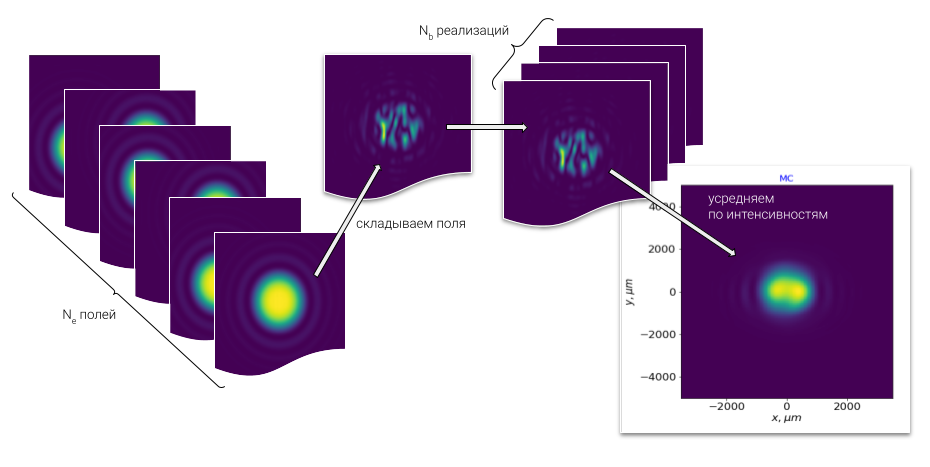
\includegraphics[width=0.99\linewidth]{MC_scheme.png}
	\caption{Схема работы метода сложения амплитуд \rr{перерисовать, изменить подпись}}
	\label{fig:SRW_scheme}
\end{figure}
\rr{сделать заметку, что чем хуже когерентности тем больше реализаций нужно, чтобы получить гладкое решение}
\noindent результирующая интенсивность будет сходиться к некоторой огибающей. В грубом приближении огибающая является свёрткой распределения расходимости излучения и распределения расходимости электронного пучка. Данный подход является наиболее прямым подходом к задаче моделирования частично когерентного излучения, однако время расчёта в таком случае может быть оценено как время затрачиваемое на расчёт одной одного поля $N_e$ раз по формуле~\ref{eq:single_electron_far_field} или~\ref{eq:single_electron_near_field}, в последней, как уже упоминалось, необходимо дважды численно взять интеграл $\textup{Ei}(\cdot)$ и потом усреднить по $N_b$ реализациям поля $\bar{E}_{b}$. Итого, если за $\tau_{calc}$ взять время расчёта одного поля, то расчёт одного результирующего поля в сумме займёт $T_{calc} = \tau_{calc} \cdot N_e \cdot N_b$.

Однако в случае полностью некогерентного излучения время расчёта можно сократить за счёт фазового фактора $\exp{(i \omega t_k)}$, который эффективно приводит к тому, что отдельный электрон в электронном пучке коррелирует только с самим собой \cite{geloni_transverse_2008}. Таким образом формула~\ref{eq:I_MC} упрощается до 
\begin{align}
 	I_{\omega} = \sum\limits_{k=1}^{N_e} \bigg|\bar{E}(\vec{\eta}_k, \vec{\l}_k, z, \vec{r}, \omega)\bigg|^2,
 	\label{eq:I_SRW} 
\end{align}
\begin{figure}[H] 
	\centering 	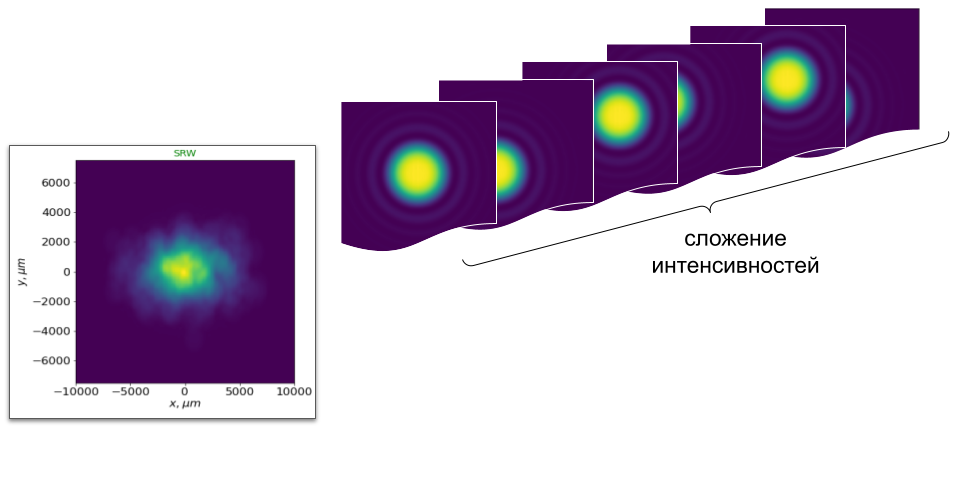
\includegraphics[width=0.99\linewidth]{SRW_scheme.png}
	\caption{Схема метода сложения интенсивностей \rr{перерисовать, изменить подпись}}
	\label{fig:SRW_scheme}
\end{figure}
\noindent а время расчёта уменьшается до $T_{calc} = \tau_{calc} \cdot N_e$. Недостатком такого подхода можно считать потерю фазовой информации о излучение и, следовательно, невозможности расчёта поперечной автокрелляционной функции первого порядка \rr{Можно ли через второй порядок найти первый? Нужна пояснительная команда}. Тем не менее, подход основанный на формуле~\ref{eq:I_SRW} даёт мощный метод расчёта частично когерентного излучения. Именно этот подход реализован в широко распространённом коде SRW \rr{cite}.
 
\subsection{Влияние размера электронного пучка на расходимость излучения}
\rr{где такой эффект можно неожиданно встретить?}

\rr{продольно когерентный случай, CSR}
\begin{figure}[H] 
	\centering 	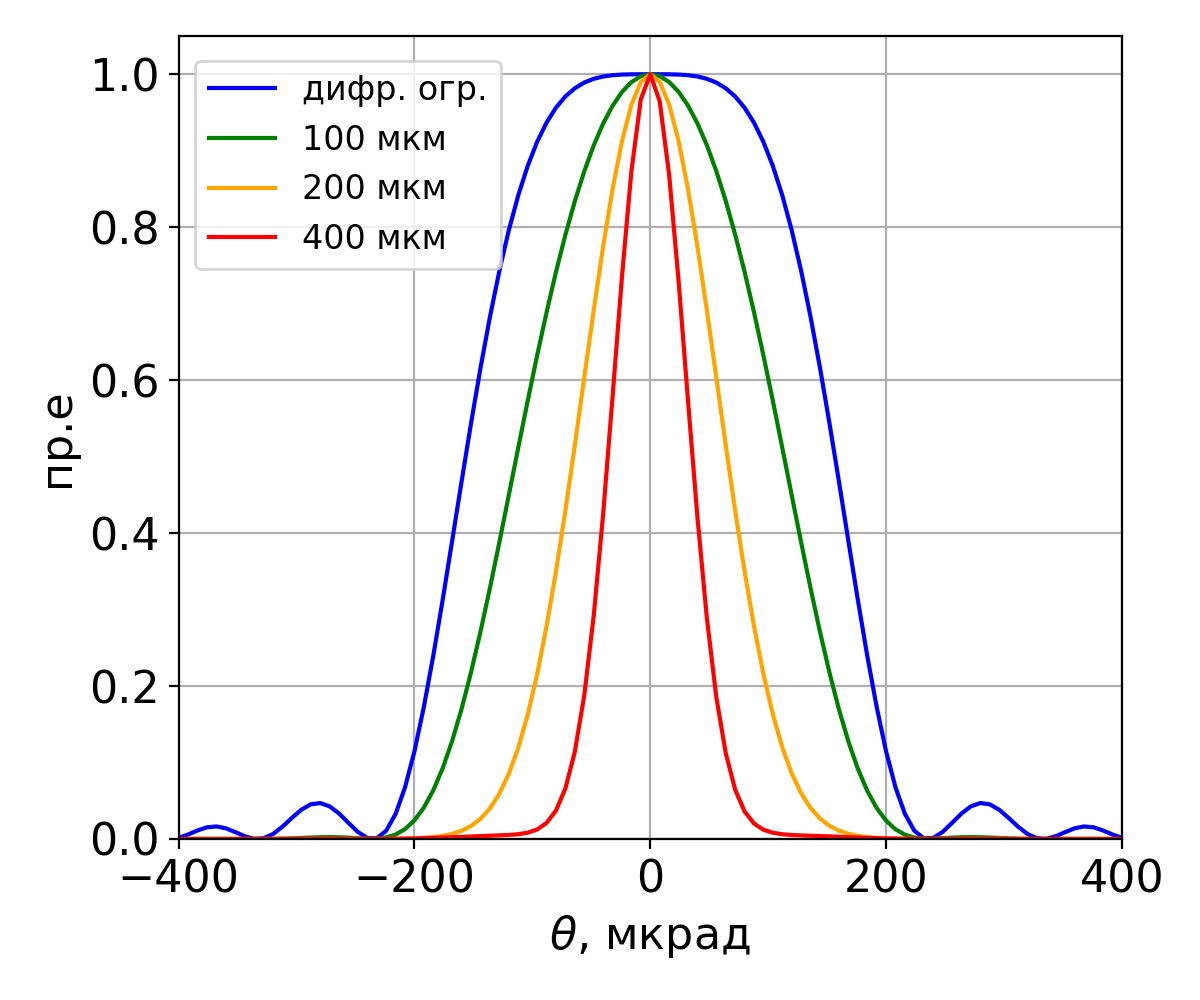
\includegraphics[width=0.99\linewidth]{diff_divergence_coh.png}
	\caption{Интенсивность комплексного гауссового шума}
	\label{fig:diff_coh_incoh_rad}
\end{figure}

\rr{некогерентный случай, варианты с различной бета-функцией}
\begin{figure}[H] 
	\centering 	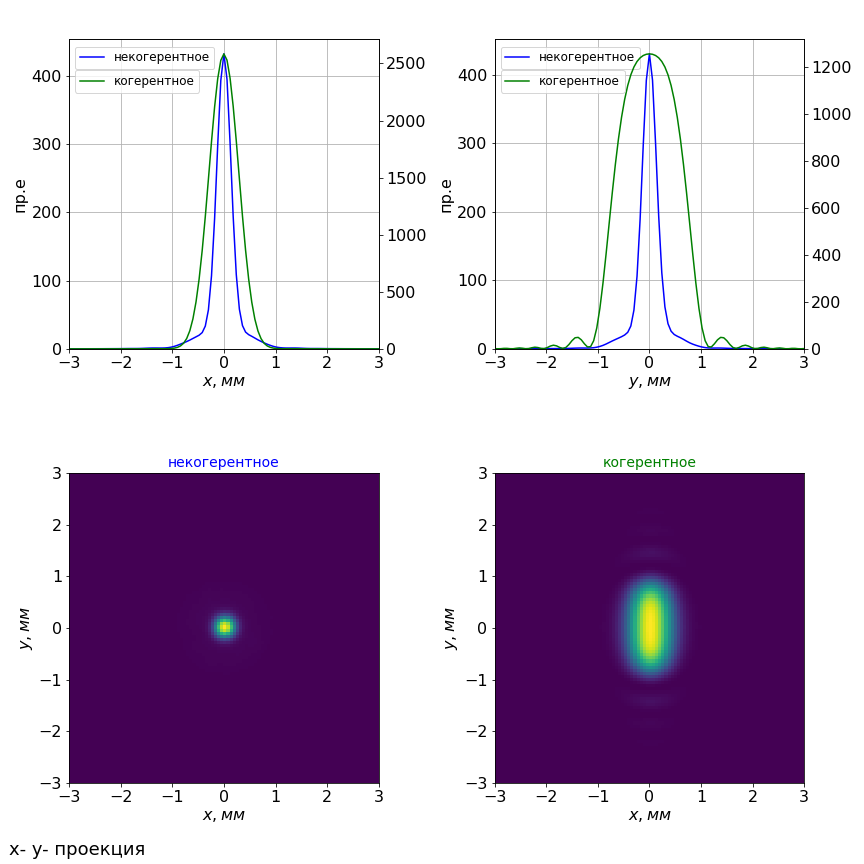
\includegraphics[width=0.99\linewidth]{diff_divergence_incoh.png}
	\caption{Интенсивность комплексного гауссового шума}
	\label{fig:diff_coh_incoh_rad}
\end{figure}

\subsection{Различие расходимости излучения для случая продольно полностью когерентного и некогерентного пучка}
В зависимости от длительности электронного пучка результирующее поле $\bar{E}_{b}$ будет вести себя по-разному. В случае короткого электронного пучка: $\omega \sigma_T \ll 1$, где $\sigma_T$ -- длительность электронного сгустка, излучение будет продольно когерентным, в иностранной литературе этот эффект называется Coherent Synchrotron Radiation (CSR). Методы моделирования такого излучения рассмотрены в работах \rr{cite}. Приближение короткого электронного пучка справедливо для низких энергий \rr{каких?}. Случай длинного электронного пучка, а именно  $\omega \sigma_T \gg 1$ соответствует случаю продольно некогерентного излучения, а для уравнения~\ref{eq:E_bunch} это означает, что показатель экспоненты $\omega \sigma_T$ равномерно распределён в интервале от $0$ до $2 \pi$. 

\rr{отличие на $\sqrt{2}$}

\rr{где такой эффект можно неожиданно встретить? Вероятнее всего на XFEL, в случае когда пучок обычный (16 фс) и скомпрессированный пучок}
\begin{figure}[H] 
	\centering 	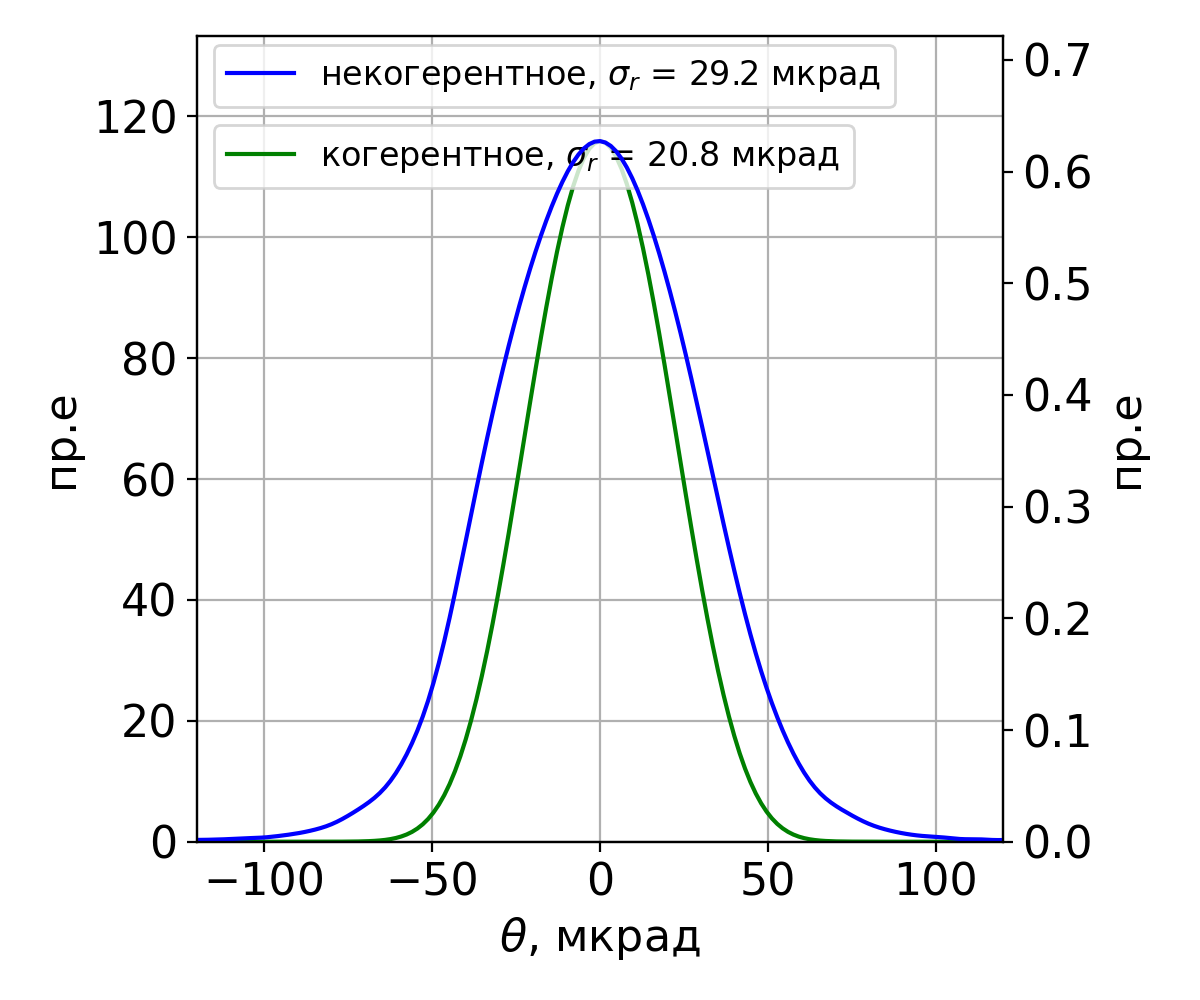
\includegraphics[width=0.99\linewidth]{diff_coh_incoh_rad.png}
	\caption{Интенсивность комплексного гауссового шума}
	\label{fig:diff_coh_incoh_rad}
\end{figure}
\section{Метод ограничения пространственных гармоник огибающими: СЕРВАЛ}
Предлагаемый метод основывается на моделировании стохастического характера ондуляторного синхротронного излучения комплексным гауссовым шумом с последующим его ограничением огибающими поля. Для начала алгоритм будет представлен в общем виде, без уточнения чем определяются распределение огибающих, задающих размер и расходимость излучения и, в целом, безотносительно характера ондуляторного источника излучение. Алгоритм создания поля представлен ниже: 
\begin{enumerate}
\item \label{noise} Создание комлексного гауссового шума $Z = X + iY$ в $r\omega$-пространстве, где величины $X$ и $Y$ подчиняются нормальному распределению.
\begin{figure}[H] 
	\centering 	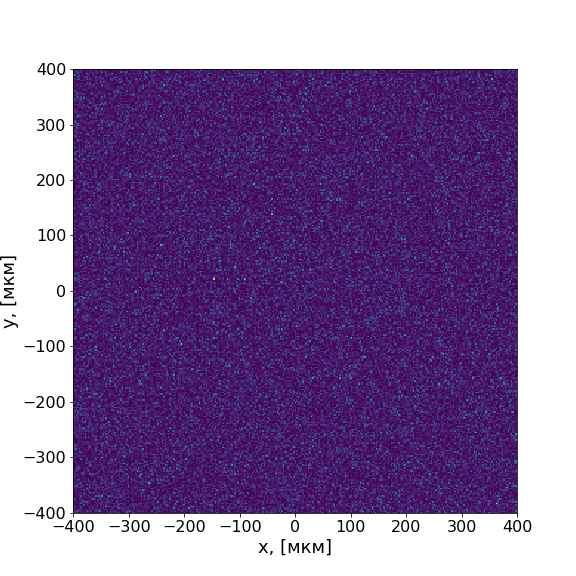
\includegraphics[width=0.45\linewidth]{1-X_noise.png}
	\caption{Интенсивность комплексного гауссового шума}
	\label{fig:1-noise}
\end{figure}
\item \label{beam_s} Ограничение шума эффективным размером электромагнитного излучения в источнике излучения в \textit{r$\omega$}-пространство.
\begin{figure}[H]
	\centering
	\begin{minipage}{0.45\textwidth}
		\centering
		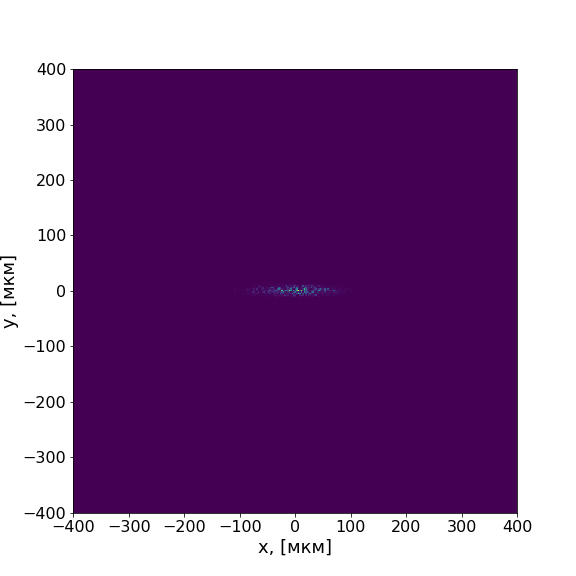
\includegraphics[width=1\linewidth]{2-X_e-beam-size.png}
		\caption{Размер электромагнитного излучения в перетяжке наложенный на шум}
		\label{fig:2-beam_size_k}
	\end{minipage}
	\begin{minipage}{0.45\textwidth}
		\centering
		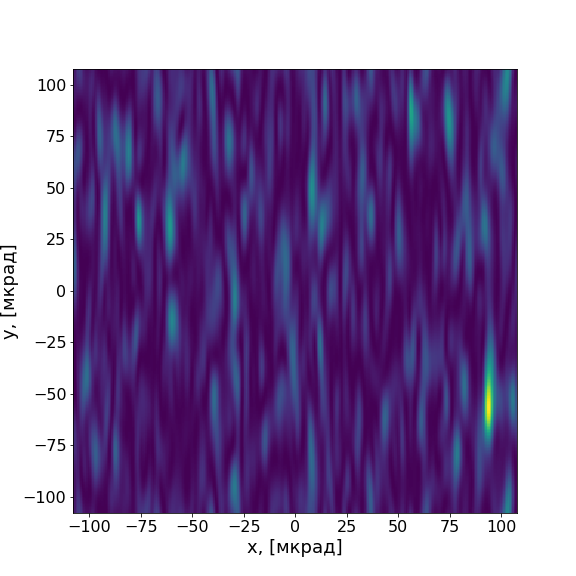
\includegraphics[width=1\linewidth]{2-X_e-beam-divergence.png}
		\caption{Получившиеся моды в $k\omega$-пространстве от размера электронного пучка}
		\label{fig:2-beam_size_s}
	\end{minipage}\hfill
\end{figure}
\item \label{beam_k} Ограничение пространственных мод эффективной расходимостью излучения в \textit{k$\omega$}-пространстве
\begin{figure}[H]
	\centering
	\begin{minipage}{0.45\textwidth}
		\centering
		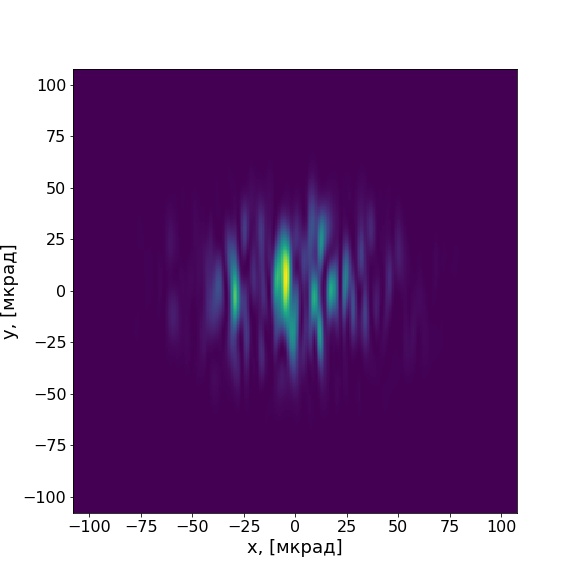
\includegraphics[width=1\linewidth]{3-X_radaition_divergence.png}
		\caption{Расходимость излучения в источнике}
		\label{fig:3-beam_s}
	\end{minipage}
	\begin{minipage}{0.45\textwidth}
		\centering
		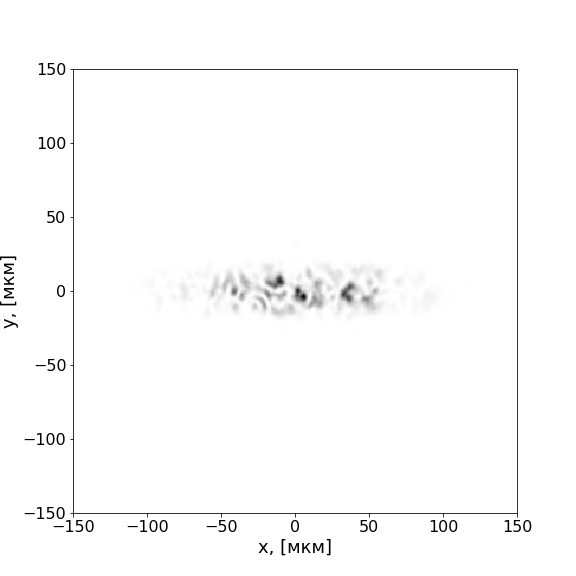
\includegraphics[width=1\linewidth]{3-X_radaition_size.png}
		\caption{Размер излучения в источнике}
		\label{fig:3-beam_k}
	\end{minipage}
\end{figure}
\item Получившиеся распространение поля есть распределение поля в источнике излучения (центр ондулятора).
\end{enumerate}
Быстродействие алгоритма можно оценить следующим образом: алгоритм генерирует $N_x \cdot N_y \cdot N_b$ случайный величин подчиняющихся распределению $Z$, где $N_b$ -- количество реализаций поля, одно Фурье преобразование поля (преобразование поля на Рис.~\ref{fig:2-beam_size_k} в поле на Рис.~\ref{fig:2-beam_size_s}) и две операции умножения на огибающие поля. Получившиеся поле, представленное на Рис.~\ref{fig:3-beam_k}, уже готово к пропагации, так как пропагатор через свободное пространство работает именно в $kf$-пространстве.
\subsection{Выбор подходящих огибающих}
До этого момента, в работе не обсуждался выбор подходящих огибающих для поля. Вопрос выбора таких огибающих сводится нахождению распределения поля в центре ондулятора. Поле в центре может быть получено, обратной пропагацией излучения из дальней зоны обратно в центр ондулятора при помощи пропагатора излучения в свободном пространстве \rr{cite}. Однако, нахождение аналитического решения уравнения Максвелла в дальней зоне от целого электронного пучка -- не тривиальная задача.  Для оценки можно предположить, что распределение поля ондуляторного излучения от электронного пучка с конечным эмиттансам, в целом, может быть представлено как свёртка распределения поля ондуляторного излучения от одного электрона с распределением фазового пространства электронного пучка.

Для SERVAL можно предложить, как минимум, три вида огибающих для пространственного распределения источника в $r$-пространстве:
\begin{enumerate}[label=\Roman*.]
	\item \label{amplitude} ${A}_{b} (\vec{r}_{\bot}) = \big(\widetilde{E}_{\bot}(0, \vec{l}, \vec{\eta}, \vec{r}_{\bot}) \ast f_l(\vec{l})\big)(\vec{l})$ \\

	\item \label{intensity} ${A}_{b} (\vec{r}_{\bot}) = \sqrt{\big(\widetilde{E}^2_{\bot}(0,  \vec{l}, \vec{\eta}, \vec{r}_{\bot}) \ast f_l^2(\vec{l})\big)(\vec{l})}$ \\

	\item \label{e-beam} ${A}_{b} (\vec{r}_{\bot}) = f_l(\vec{l})$,
\end{enumerate}
и три вида огибающих для распределения расходимости источника ($k$-пространство):
\begin{enumerate}[label=\Roman*.]
	\item \label{amplitude} $\hat{{A}}_{b} (\vec{\theta}_{\bot}) = \big(\hat{\widetilde{E}}_{\bot}(0,  \vec{l}, \vec{\eta}, \vec{\theta}_{\bot}) \ast \hat{f}_{\eta}(\vec{\eta})\big)(\vec{\eta})$\\
	
	\item \label{intensity} $\hat{{A}}_{b} (\vec{\theta}_{\bot}) = \sqrt{\big(\hat{\widetilde{E}^2}_{\bot}(0,  \vec{l}, \vec{\eta}, \vec{\theta}_{\bot}) \ast \hat{f_{\eta}^2}(\vec{\eta})\big)(\vec{\eta})}$\\
	
	\item \label{e-beam} $\hat{{A}}_{b} (\vec{\theta}_{\bot}) = \hat{f}_{\eta}(\vec{\eta})$,
\end{enumerate}
где ${A}_{b} (\vec{r})$ и $\hat{{A}}_{b} (\vec{\theta})$ огибающие в $r$- и $k$-пространствах соответствующие шагам~\ref{beam_s} и~\ref{beam_k} в алгоритме,  $f(\vec{l}, \vec{\eta}) = f_l(\vec{l}) f_{\eta}(\vec{\eta})$ фазовое распределение электронного пучка, и поле $\widetilde{E}_{\bot}(z=0, \vec{\l}, \vec{\eta}, \vec{r}_{\bot})$, $\hat{\widetilde{E}}_{\bot}(z=0 , \vec{\l}, \vec{\eta}, \vec{\theta}_{\bot})$ -- распределение поля взятого в центре ондулятора по формулам \ref{eq:single_electron_far_field}(или более точно \ref{eq:single_electron_near_field}) и \ref{eq:single_electron_near_field_z=0}.

Для выбора подходящих амплитуд было проведено моделирование с различными огибающими в сравнение с эталонным в этой работе методом сложения амплитуд. Для начала необходимо проверить распределение интенсивности поля на источнике. Для метода сложения амплитуд поле было рассчитано в дальней зоне и отпропагировано назад в центр ондулятора. Результаты сравнения приведены на Рис.~\ref{fig:SERVAL_envelopes_comparison_far_zone} при параметрах электронного пучка \rr{параметры электронного пучка}
\begin{figure}[H] 
	\centering 	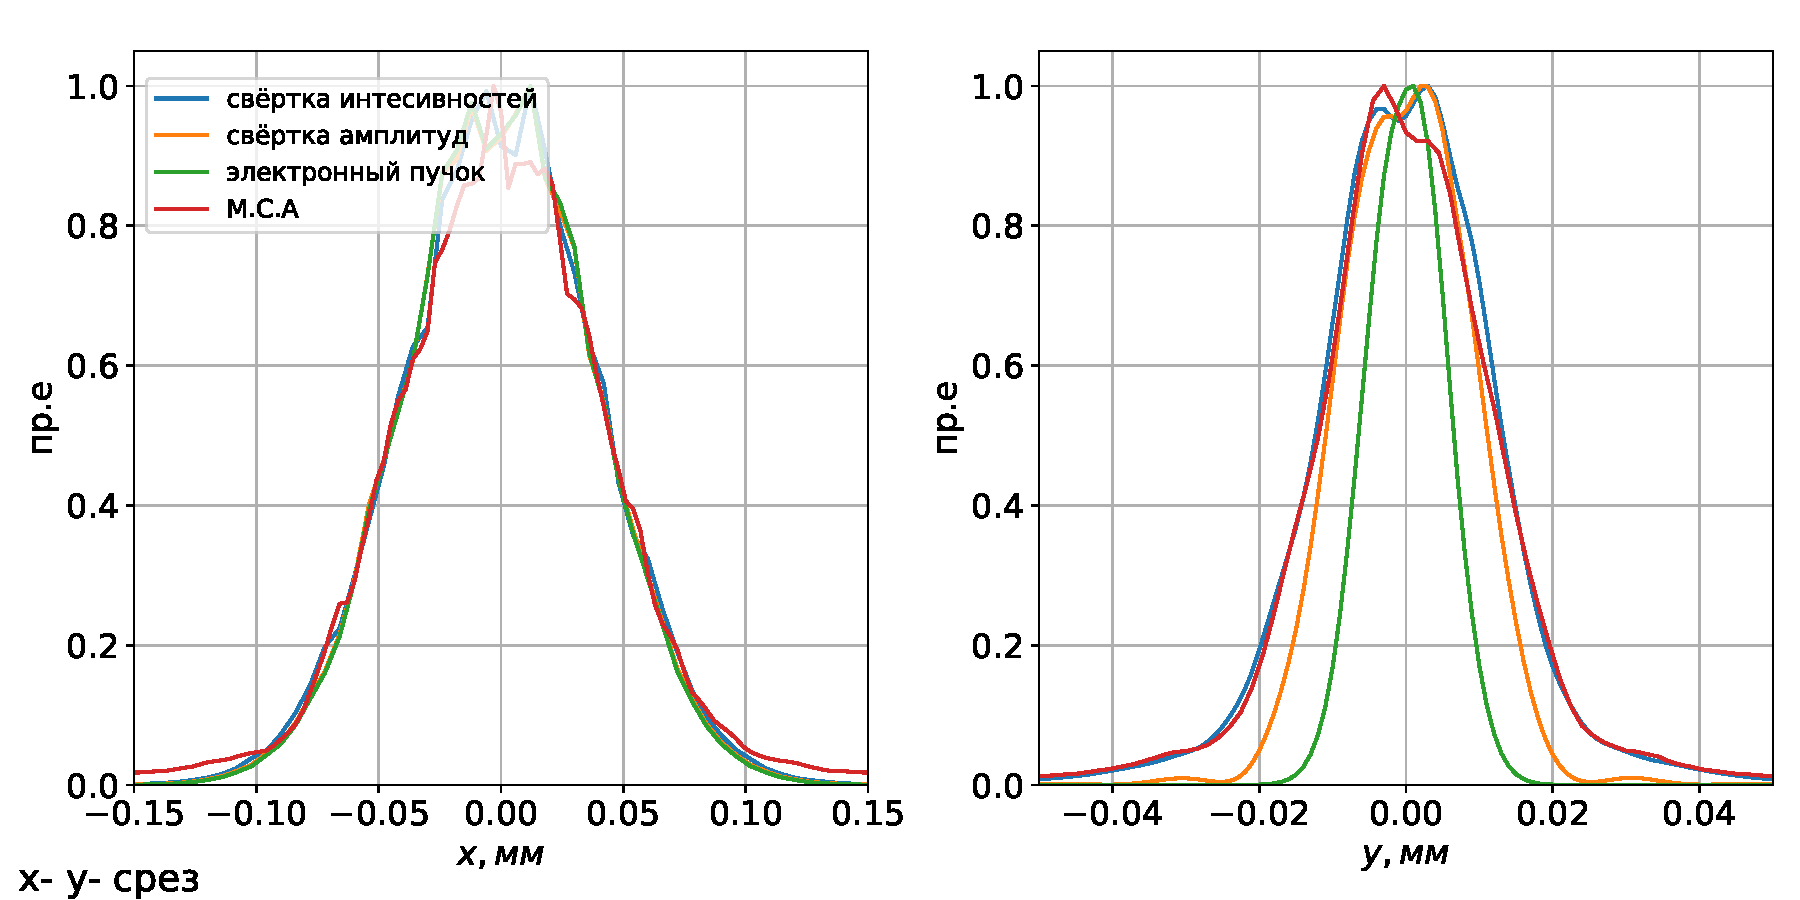
\includegraphics[width=0.99\linewidth]{SERVAL_envelopes_comparison_source.pdf}
	\caption{Распределение поля в источнике излучения}
	\label{fig:SERVAL_envelopes_comparison_far_zone}
\end{figure}
Видно, что оптимальные результаты достигаются при использовании свёртки~\ref{intensity}. Однако, если $N \ll 1$ или даже просто $N > 1$, то можно использовать любые из представленных огибающих для $r$-пространства. Необходимо так же сравнить корреляционные функции получившихся полей~\ref{fig:diff_coh_incoh_rad}, используя формулу~\ref{eq:g1}.
\begin{figure}[H] 
	\centering 	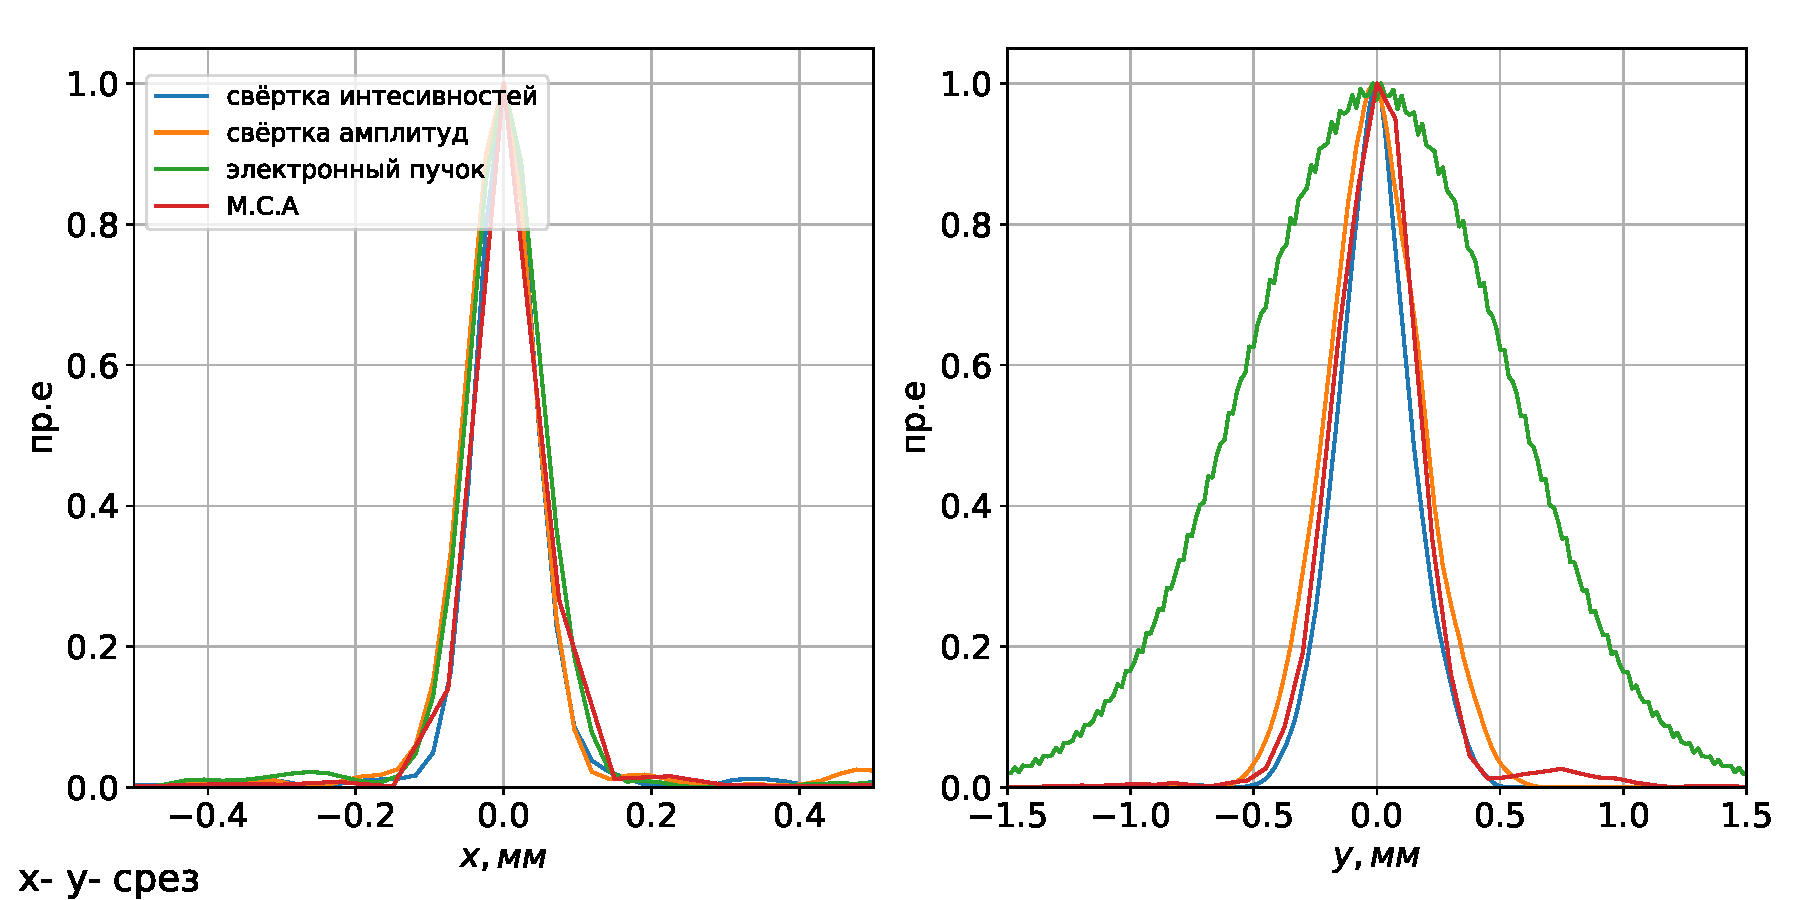
\includegraphics[width=0.99\linewidth]{SERVAL_corr_comparison.pdf}
	\caption{Функция взаимной когерентности на расстоянии $25$ м от источника}
	\label{fig:SERVAL_corr_comparison}
\end{figure}
Для распределения расходимости следует так же использовать использовать свёртку интенсивностей.
\begin{figure}[H] 
	\centering 	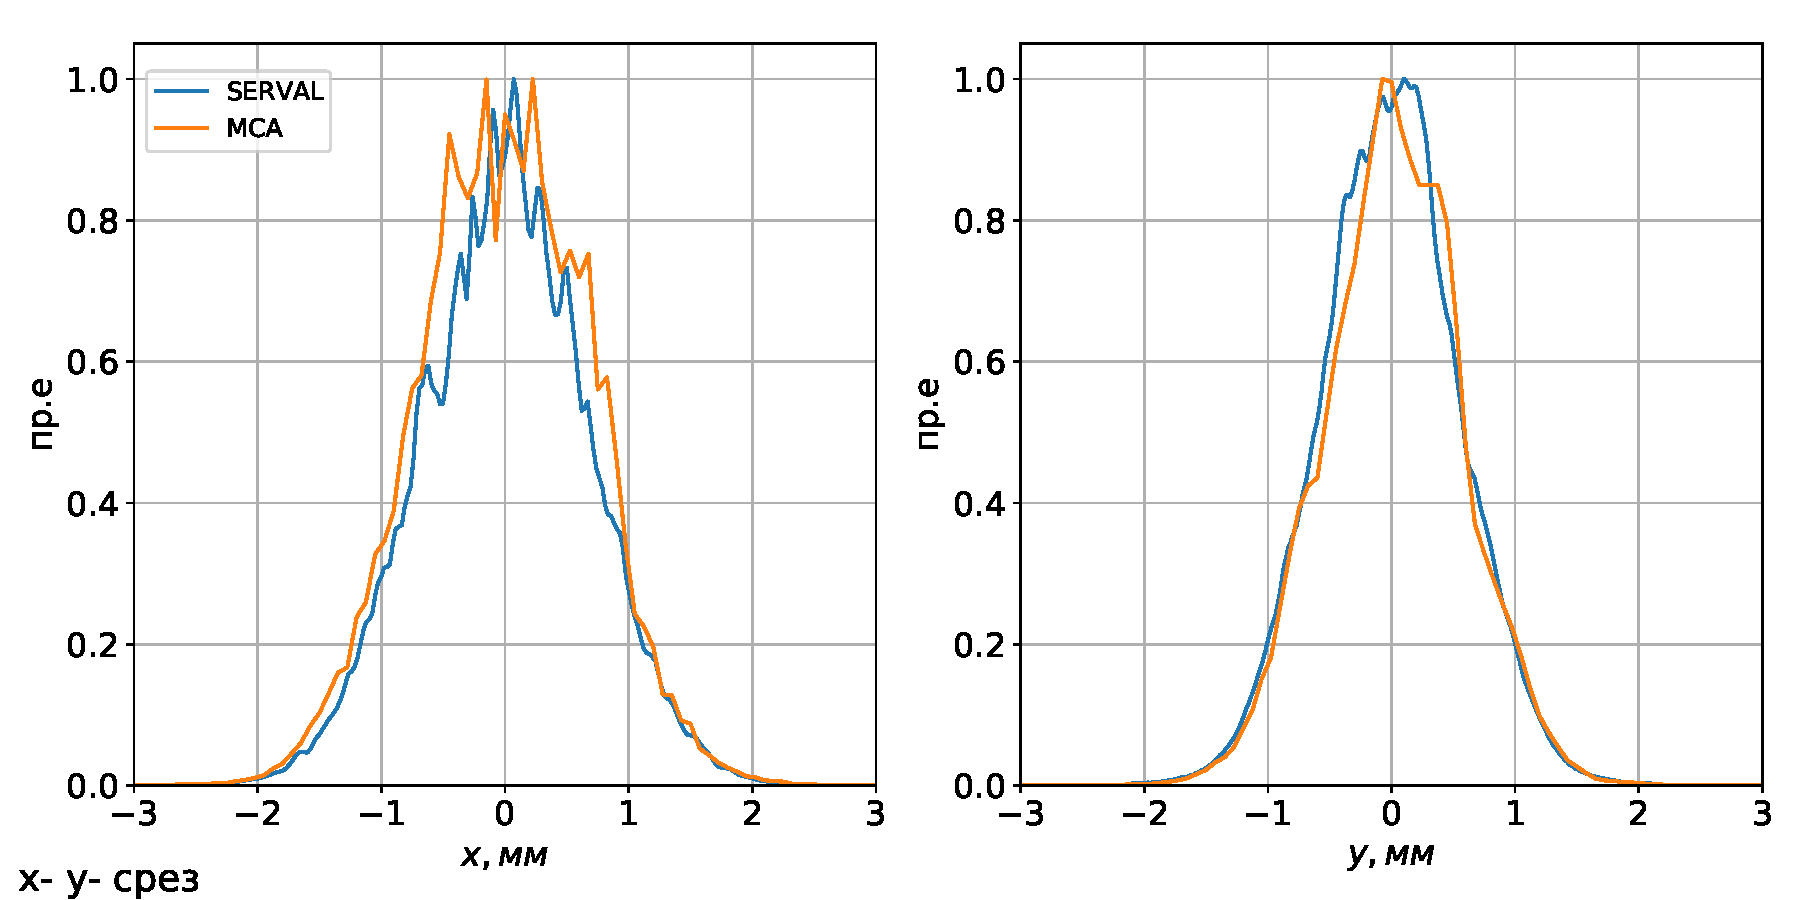
\includegraphics[width=0.99\linewidth]{SERVAL_envelopes_comparison_far_zone.pdf}
	\caption{Распределением на источнике}
	\label{fig:diff_coh_incoh_rad}
\end{figure}
В большинстве случаев можно выбирать свёртку интенсивностей по~\ref{intensity}. Однако, стоит отметить, что SERVAL -- это оценочный метод и в случаее дифракционного ограниченного источника необходимо перед проведением расчётов сделать подобный анализ подходящих огибающих. 

\chapter{Применение СЕРВАЛа}
СЕРВАЛ является эффективным алгоритмом для моделирования именно частично когерентного синхротронного излучения. Дело в том \rr{дописать в чём тут дело}. В случае дифракционно ограниченных источников, целесообразно применять метод сложения амплитуд или метод сложения интенсивностей, которые очень быстро дадут сходимость. В случае же источников с низкой степенью когерентности имеет смысл рассмотреть метод трассировки лучей. Однако, в каждом из рассмотренных случаев прежде чем проводить оптический расчёт, необходимо детально изучить свойства источника излучения и рассчитать ожидаемую степень когерентности и только исходя из свойств источника применять один из описанных методов моделирования. При описании алгоритма мы использовали параметры электронного пучка и ондулятора ЦКП «СКИФ», в этой главе мы продолжи рассмотрим применение СЕРВАЛа для частично когерентных источников излучения на примере нескольких оптических схем.

\section{Фокусирующая система}
Рассмотрим оптическую систему состоящую из источника излучения -- ондулятора, апертуры и фокусирующего элемента, делающего изображение в фокальной плоскости. Для SERVAL были выбраны огибающие~\ref{intensity}. Этот расчёт будет сопровождаться сравнением результатов SERVAL с результатами метода сложения амплитуд.

Распределение поля в дальней зоне на 25 м от ондулятора представлено на Рис.~\ref{fig:focusing_system_far_zone}.
\begin{figure}[H] 
	\centering 	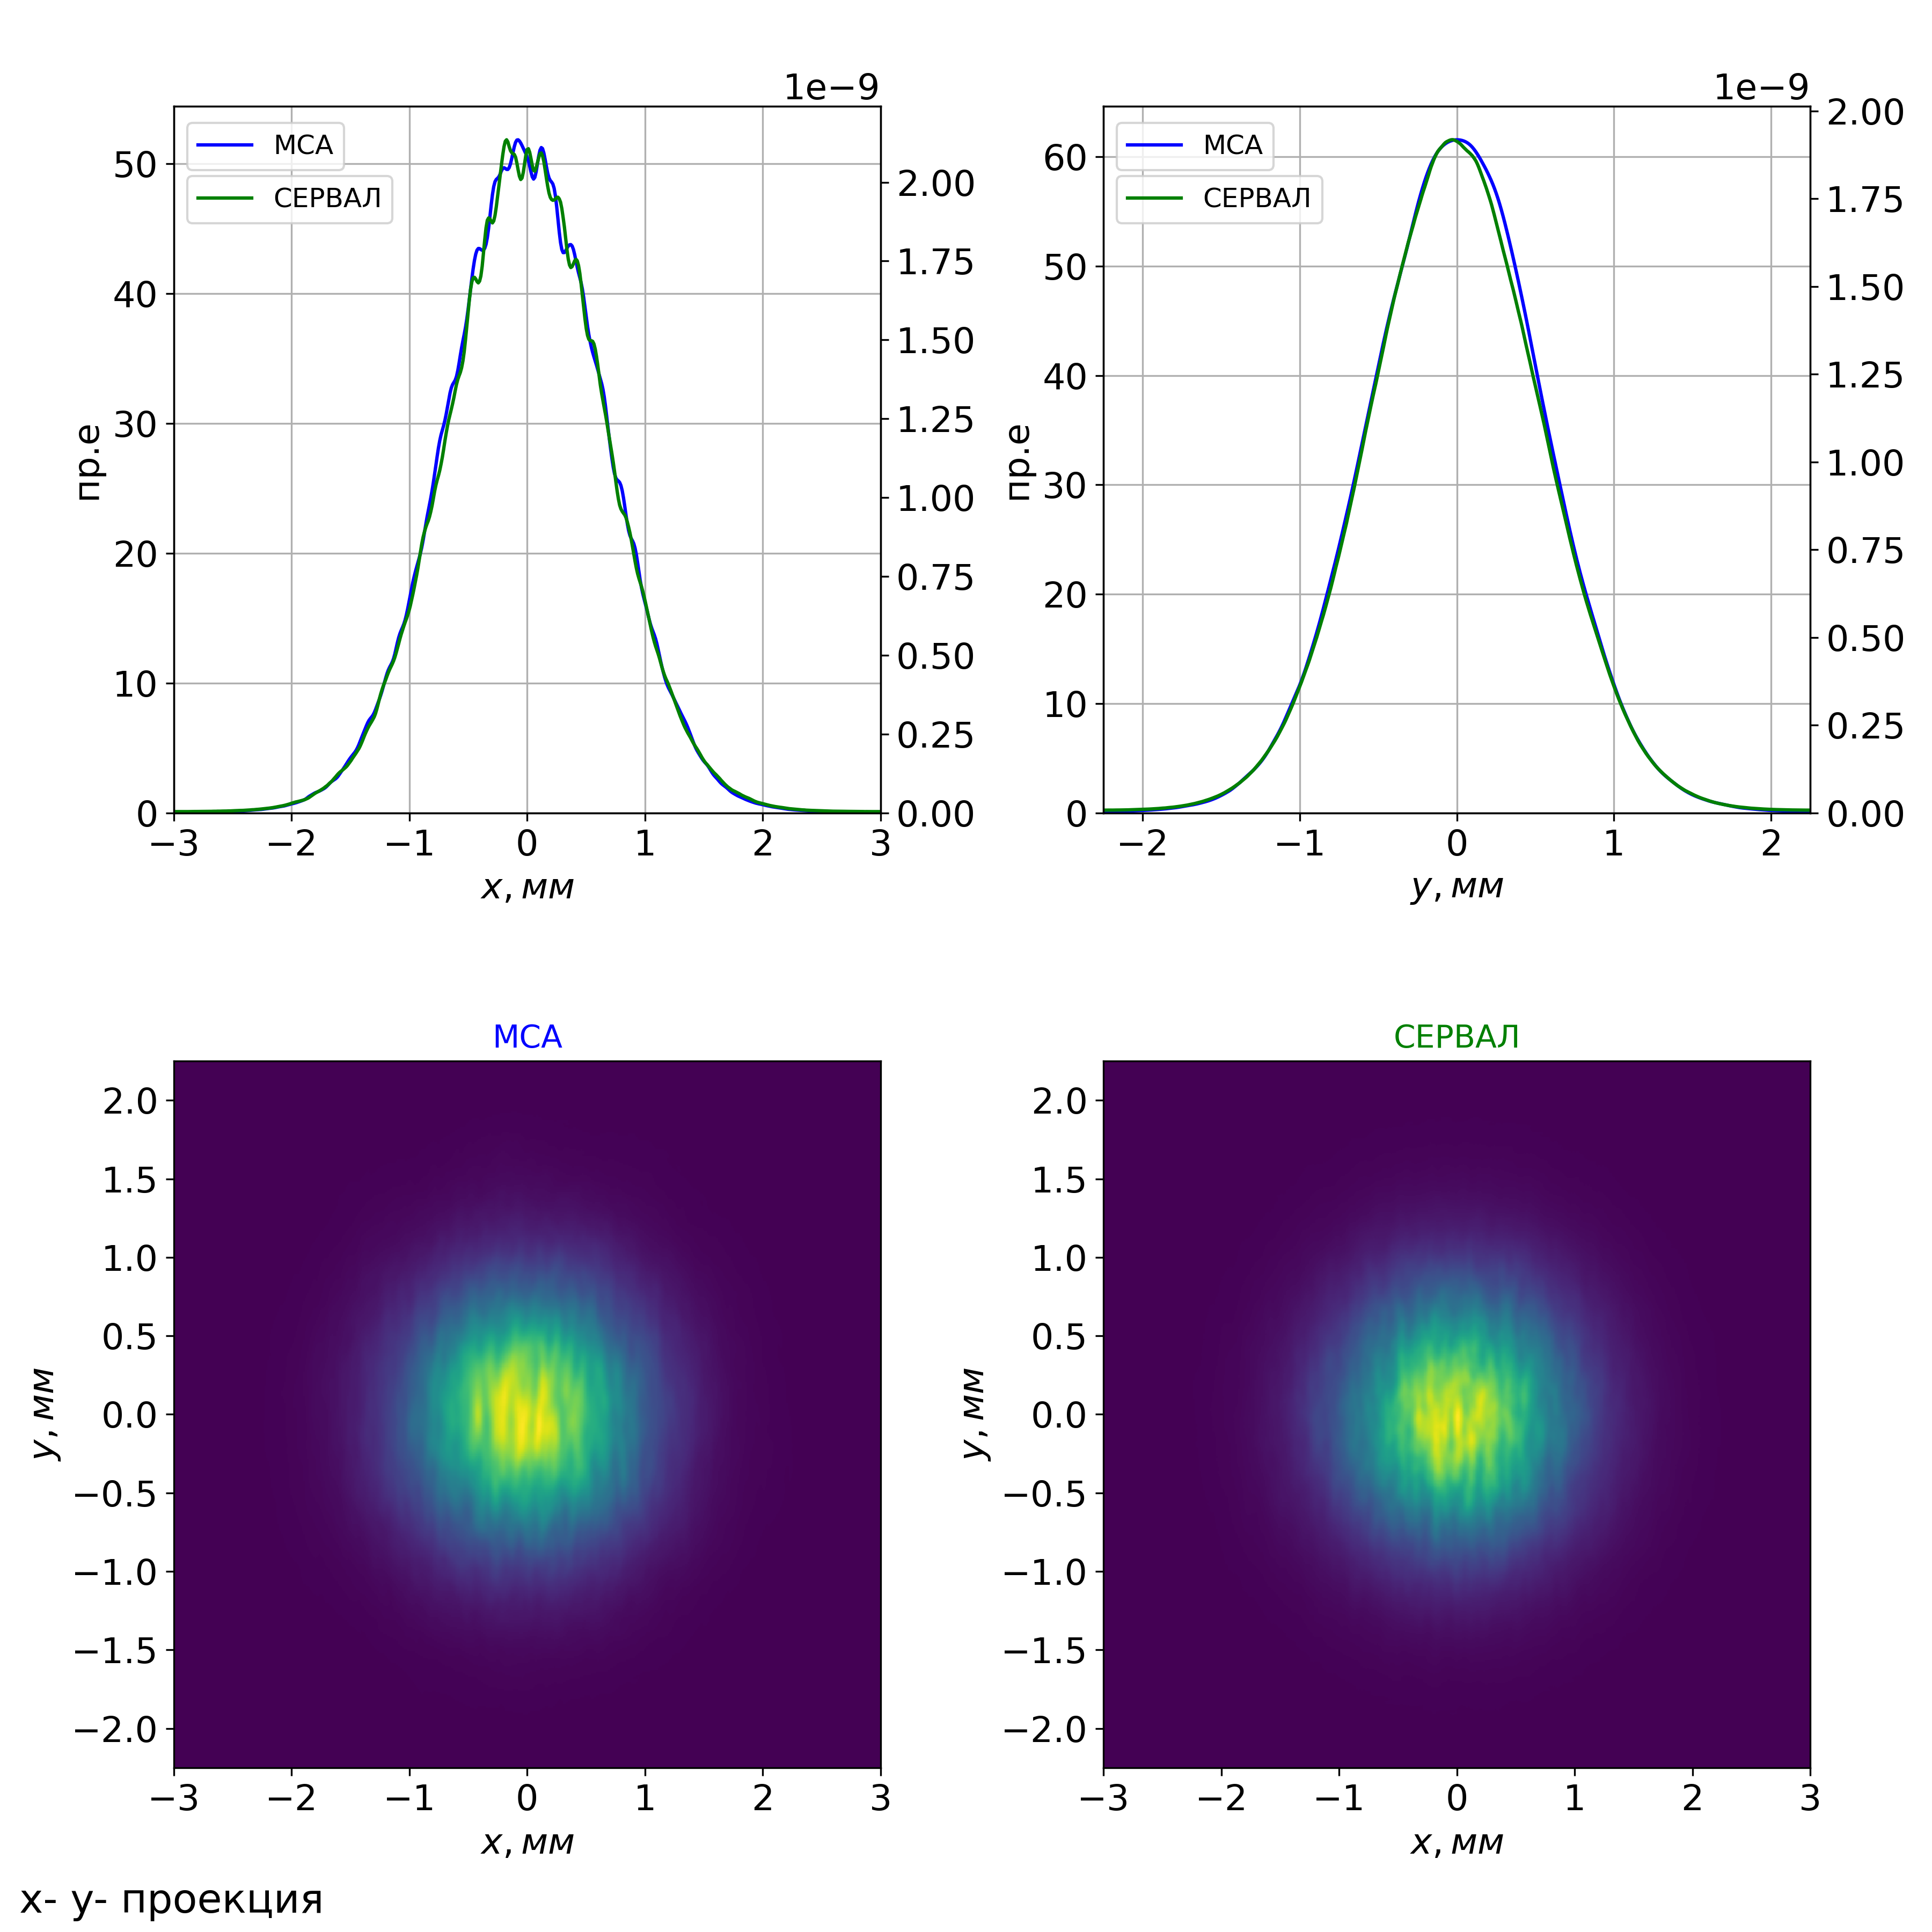
\includegraphics[width=0.99\linewidth]{1-far_zone_25_m3.80E-05_um_4.68E-06_um_2.50E-05_urad_2.00E-05_urad_example_beamline.png}
	\caption{\rr{caption, remove captions in Russian}}
	\label{fig:focusing_system_far_zone}
\end{figure}

\begin{figure}[H] 
	\centering 	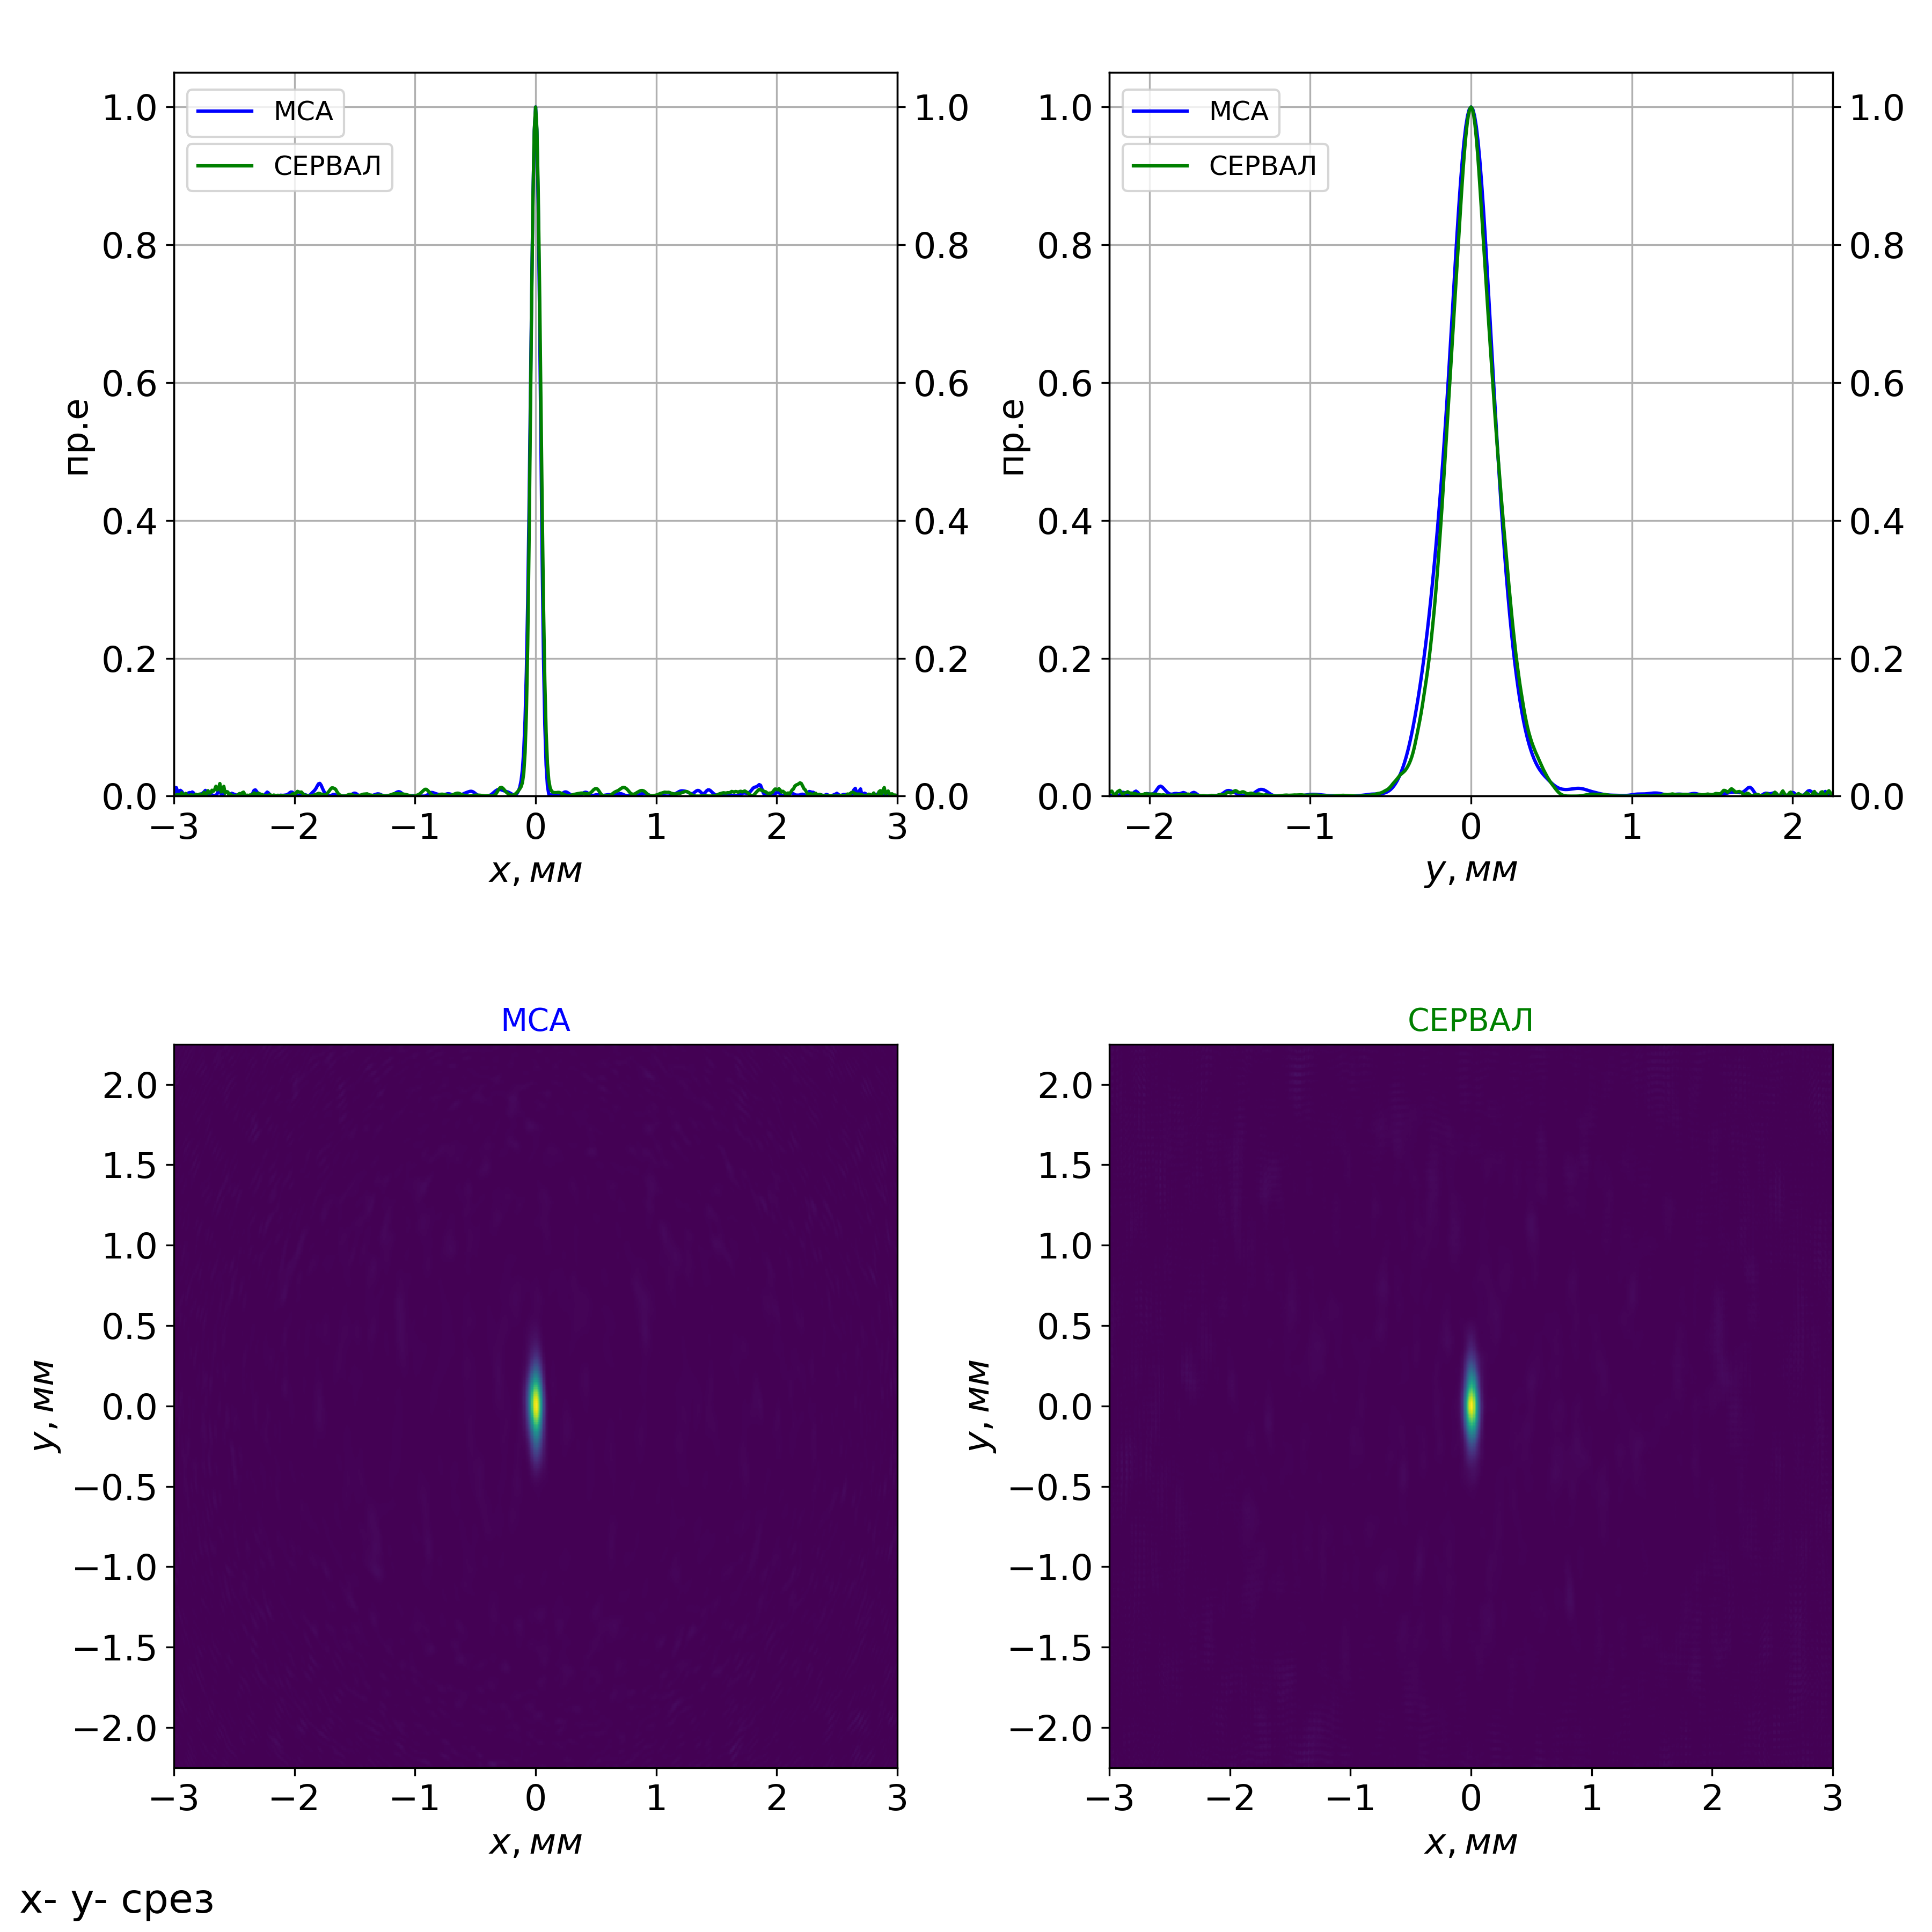
\includegraphics[width=0.99\linewidth]{corr3.80E-05_um_4.68E-06_um_2.50E-05_urad_2.00E-05_urad_example_beamline.png}
	\caption{\rr{caption, remove captions in Russian}}
	\label{fig:focusing_system_corr}
\end{figure}
\noindent После апертуры и 10 метров распространения поля через пустое пространство результат приведен на Рис.~\ref{fig:focusing_system_far_zone}
\begin{figure}[H] 
	\centering 	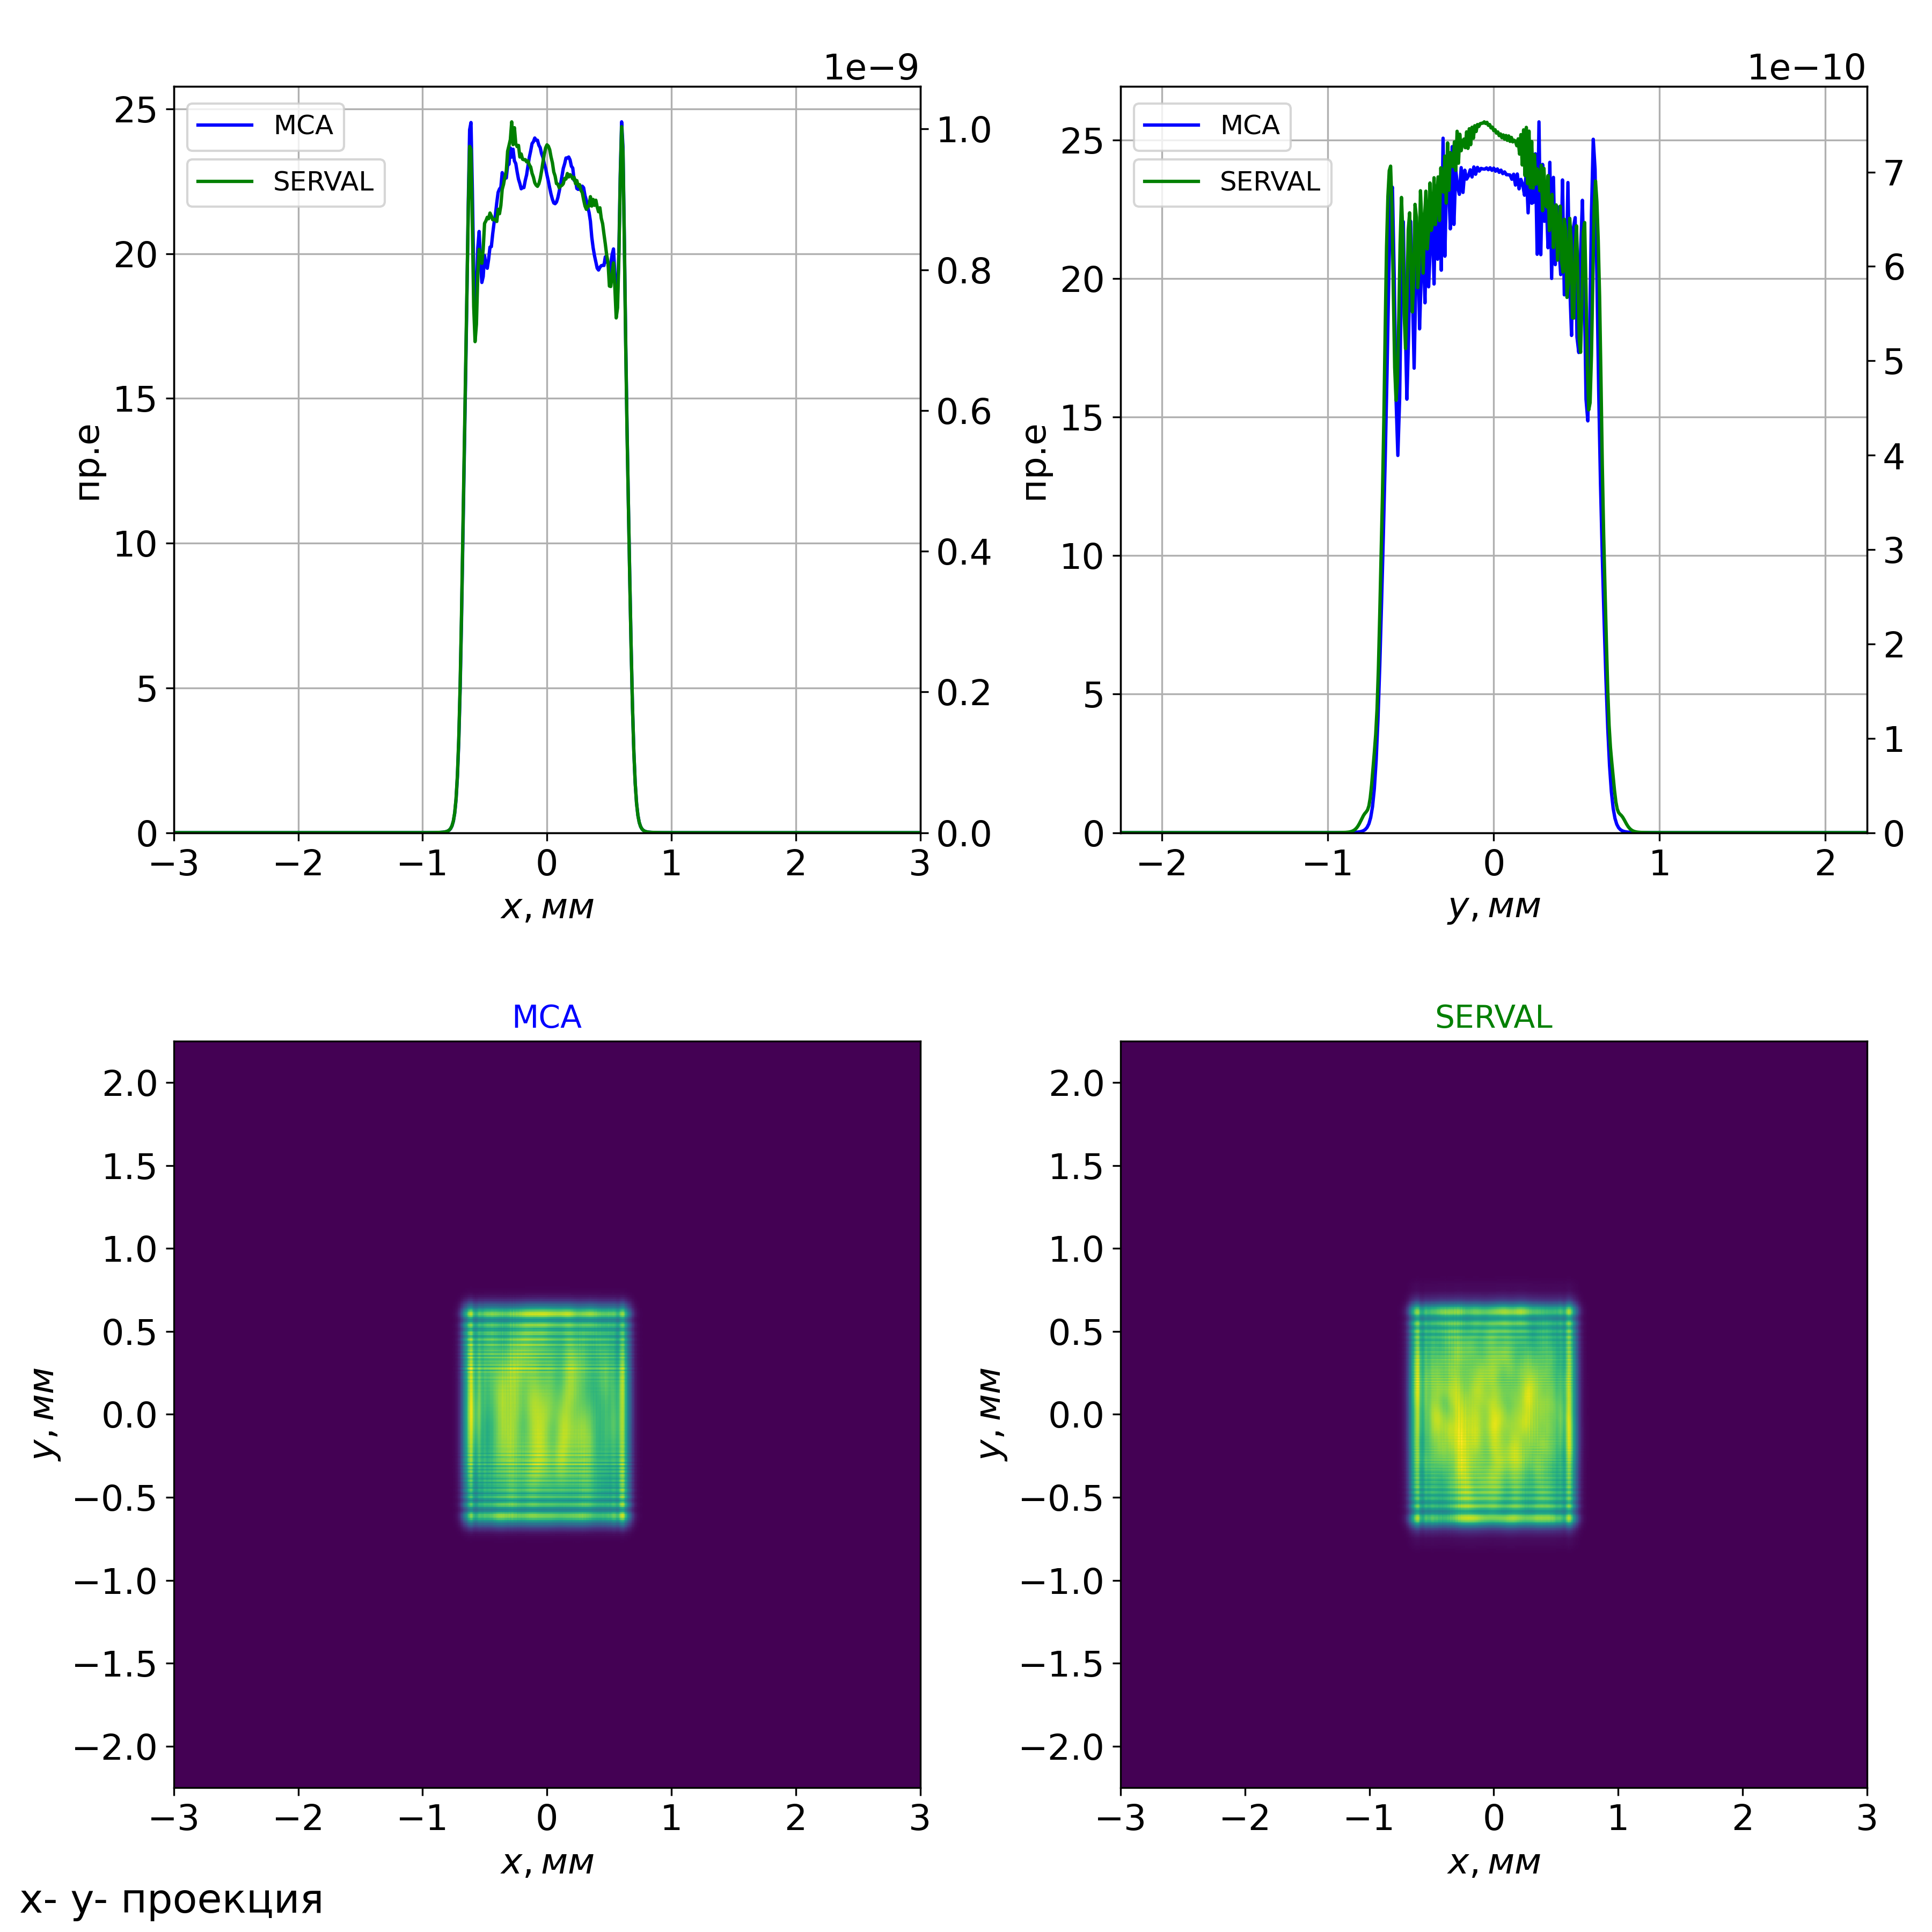
\includegraphics[width=0.99\linewidth]{2-far_zone_60_m_after_aperture3.80E-05_um_4.68E-06_um_2.50E-05_urad_2.00E-05_urad_example_beamline.png}
	\caption{\rr{caption, remove captions in Russian}}
	\label{fig:focusing_system_after_aperture}
\end{figure}
\noindent Распределение поля в фокальной плоскости приведено на Рис.~\ref{fig:focusing_system_in_focus}
\begin{figure}[H] 
	\centering 	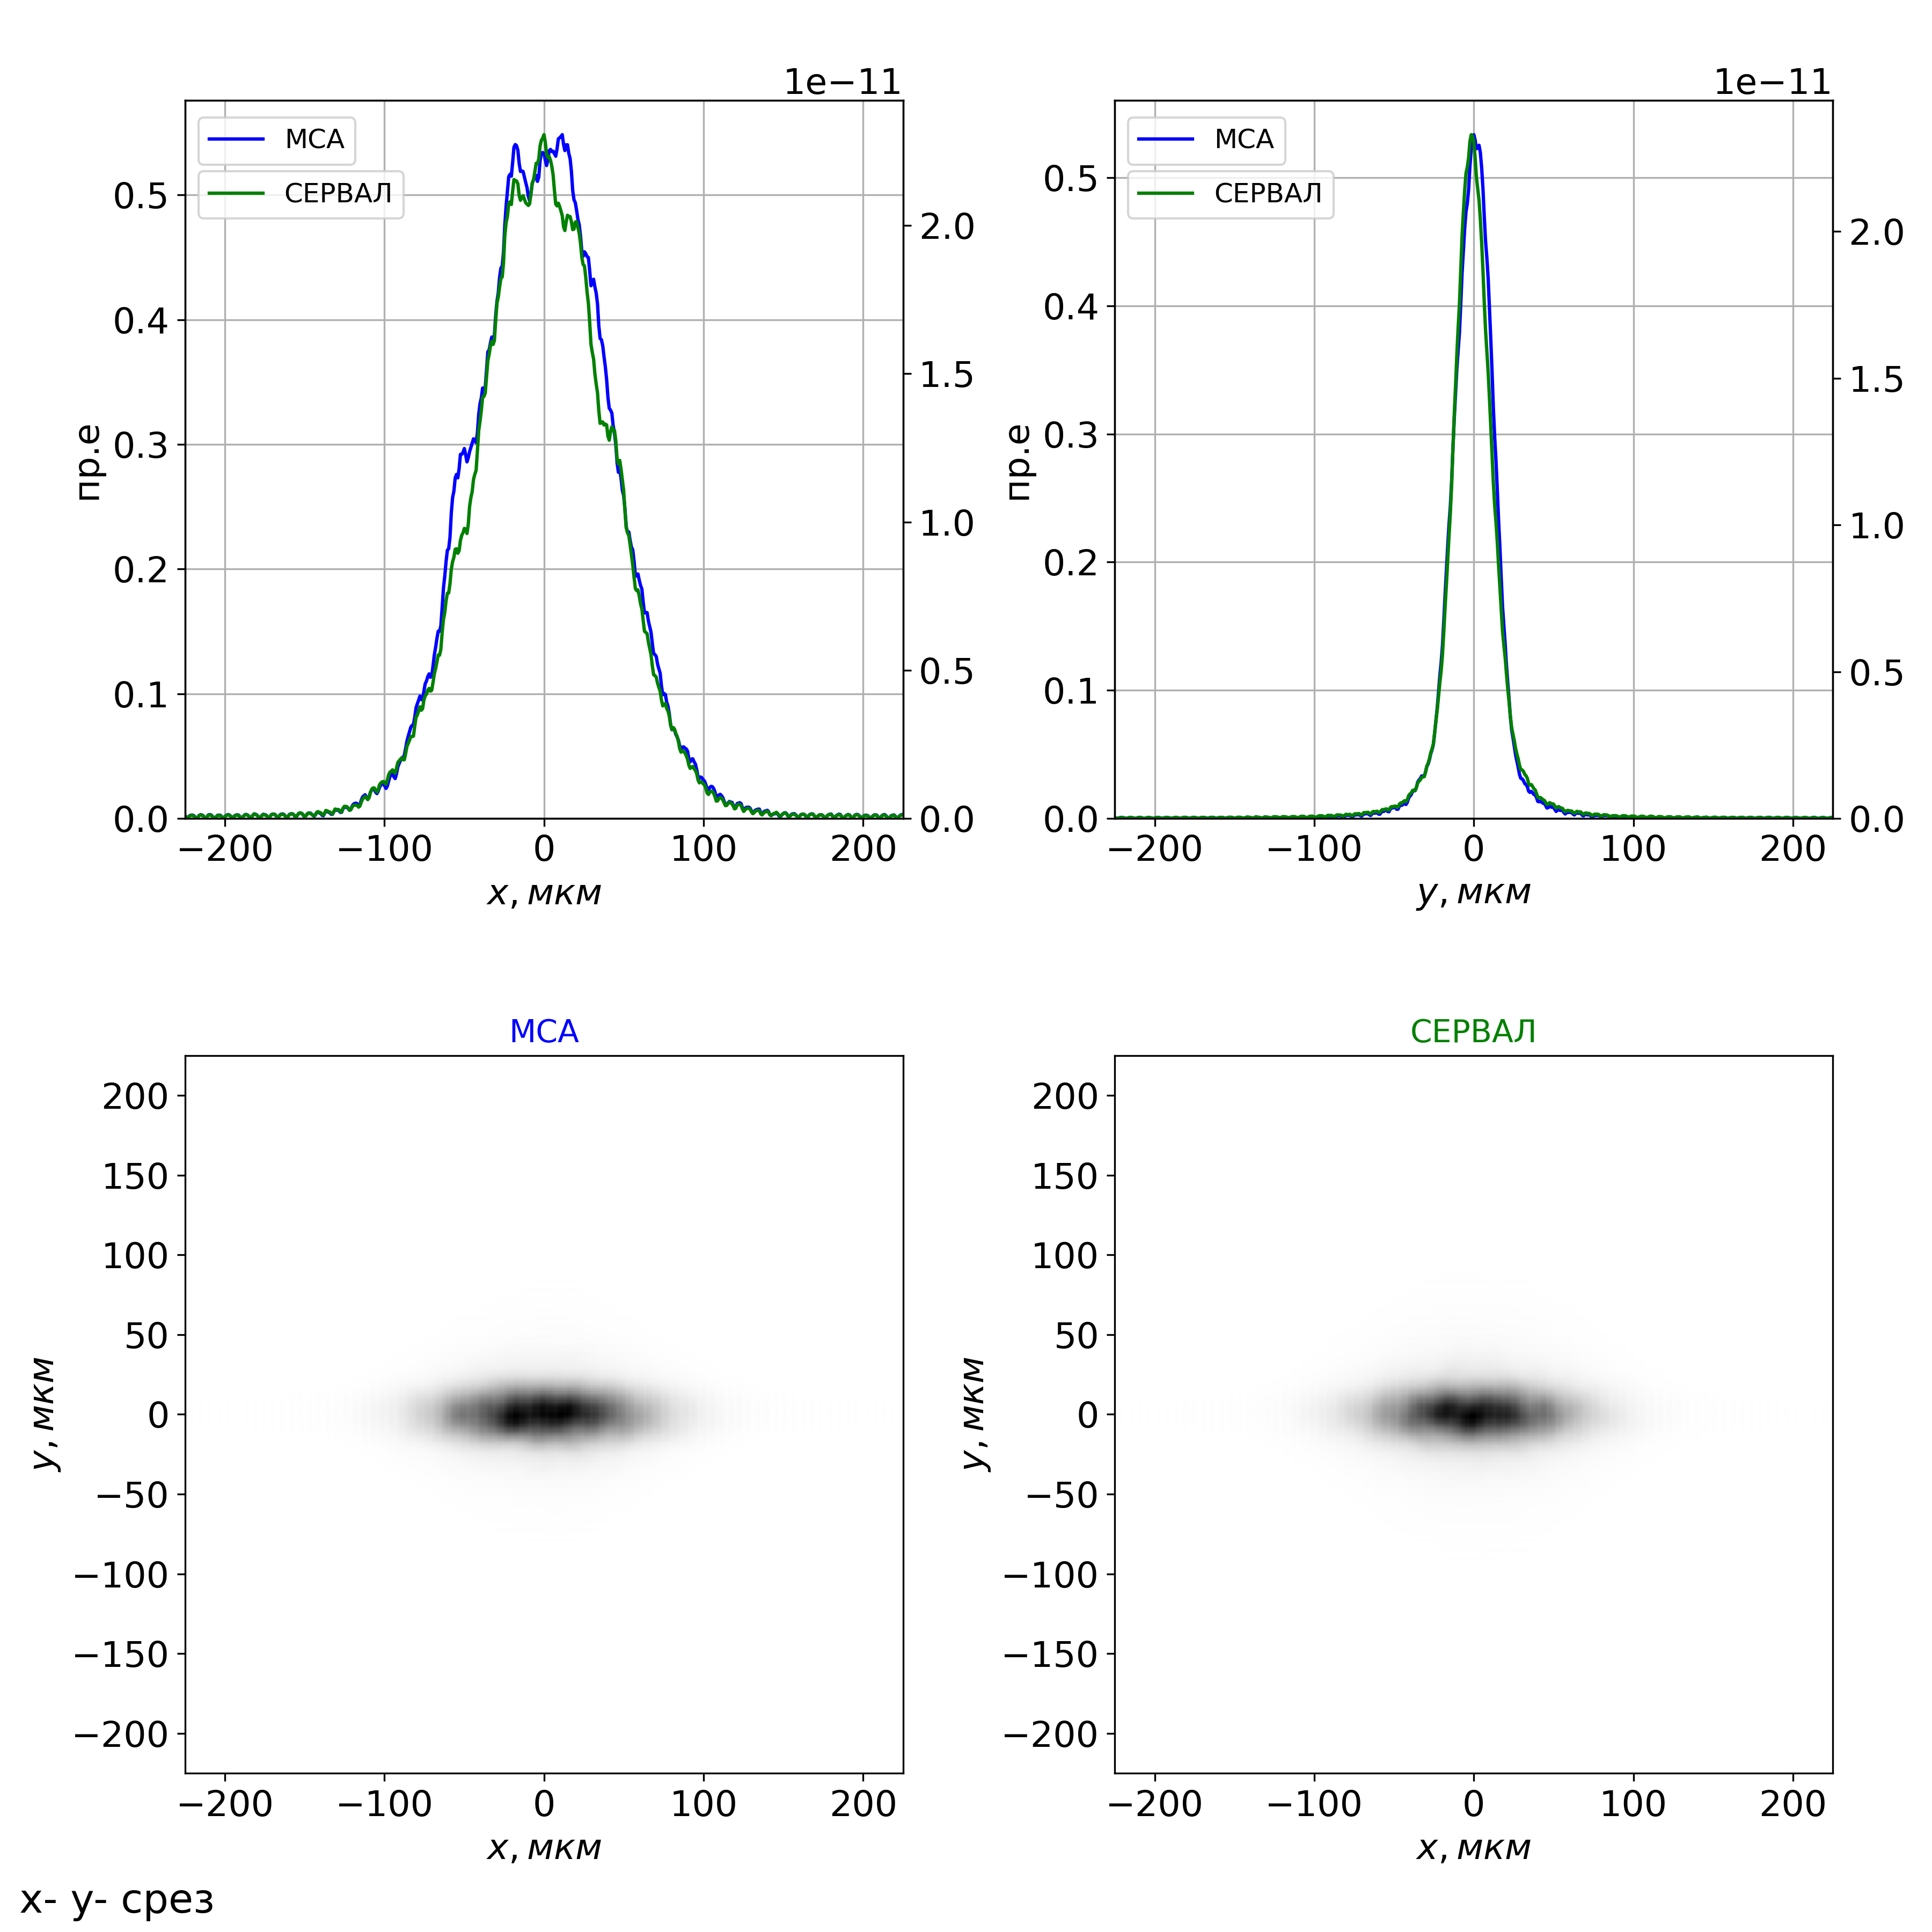
\includegraphics[width=0.99\linewidth]{3-70_m_focal_plane3.80E-05_um_4.68E-06_um_2.50E-05_urad_2.00E-05_urad_example_beamline.png}
	\caption{\rr{caption, remove captions in Russian}}
	\label{fig:focusing_system_in_focus}
\end{figure}

\subsection{Интерференционный эксперимент}

\begin{figure}[H]
	\centering
	\begin{minipage}{0.33\textwidth}
		\centering
		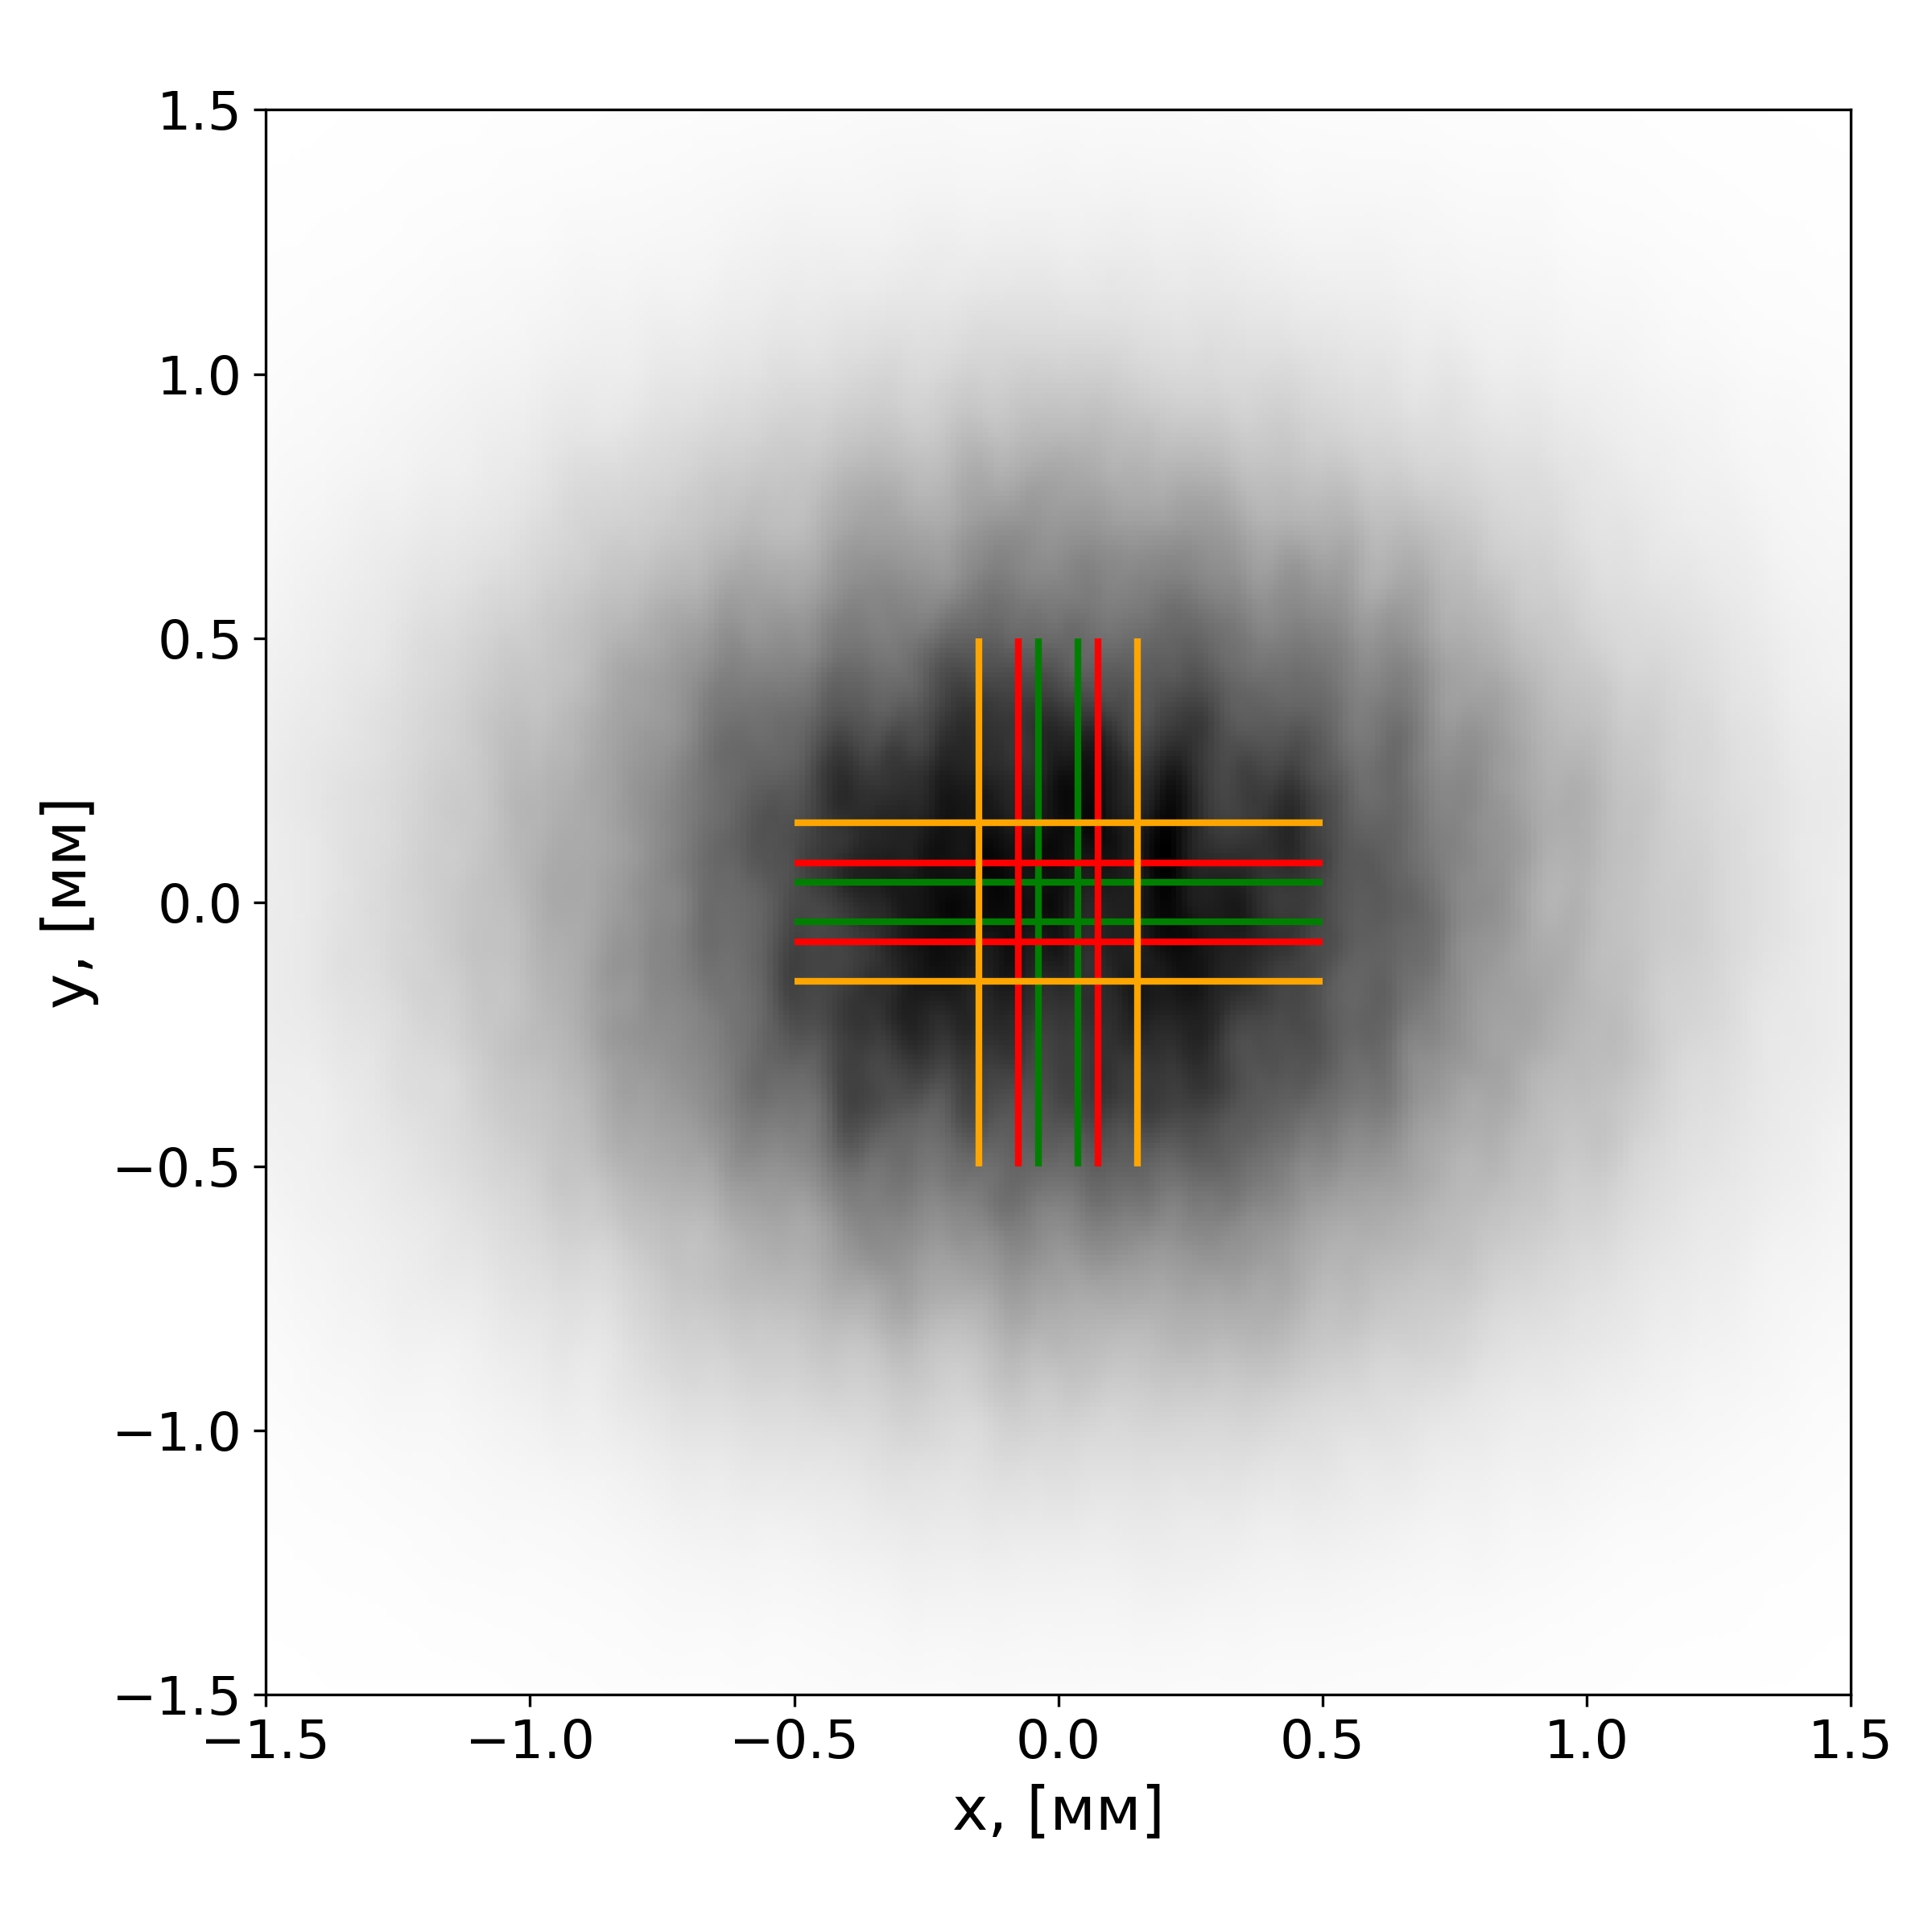
\includegraphics[width=1\linewidth]{field_before_slit.png}
		\caption{}
		\label{fig:2-beam_size_k}
	\end{minipage}
	\begin{minipage}{0.33\textwidth}
		\centering
		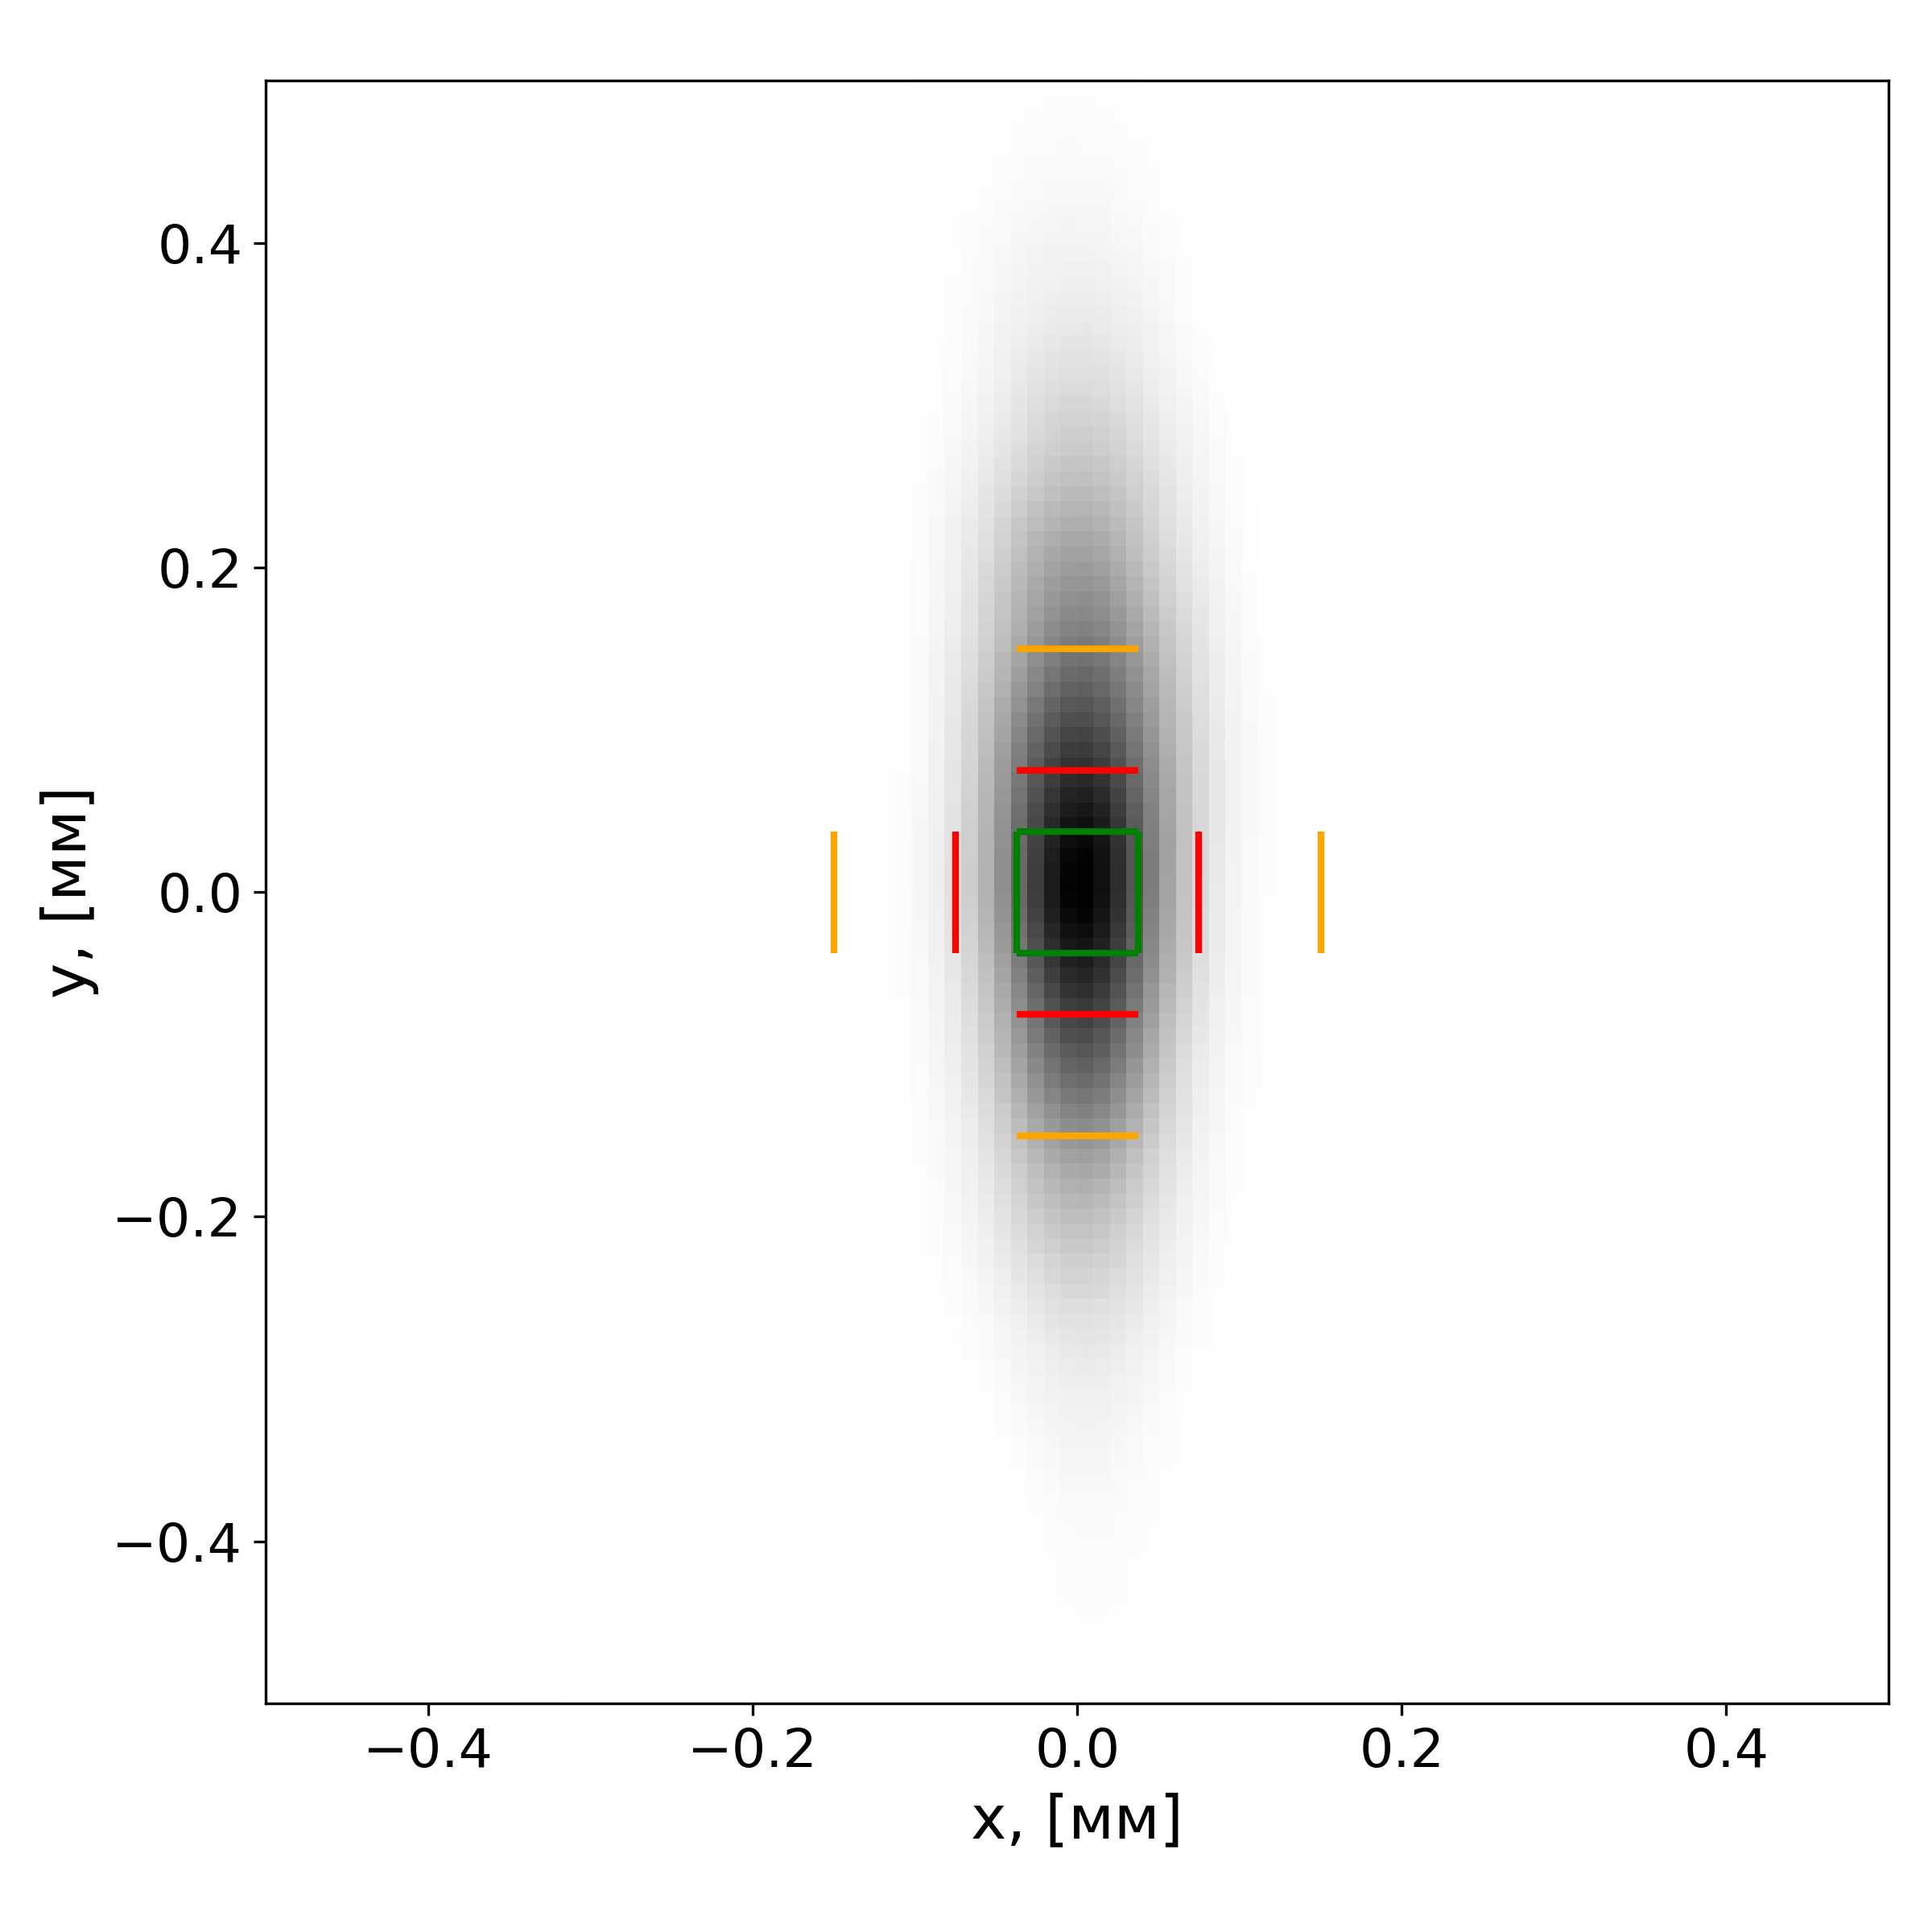
\includegraphics[width=1\linewidth]{corr_before_slit.png}
		\caption{}
		\label{fig:2-beam_size_s}
	\end{minipage}\hfill
\end{figure}

\begin{figure}[H]
	\centering
	\begin{minipage}{0.33\textwidth}
		\centering
		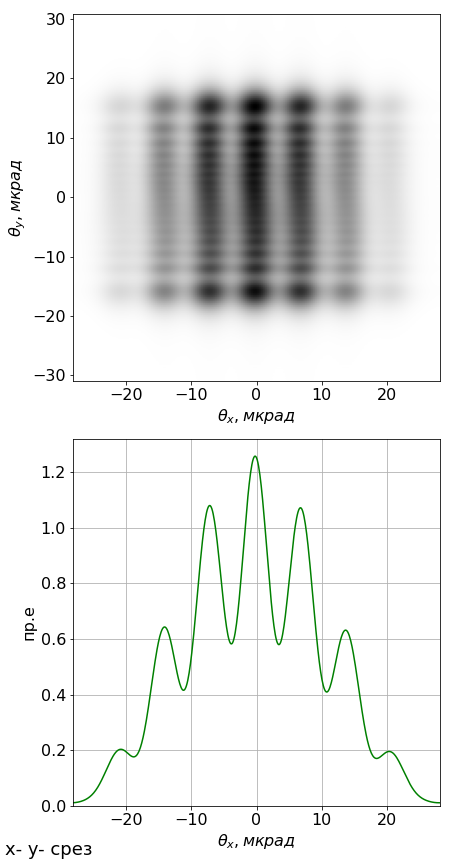
\includegraphics[width=1\linewidth]{x_slits_width_3e-05_separation_7.5e-05_.png}
		\caption{}
		\label{fig:2-beam_size_k}
	\end{minipage}
	\begin{minipage}{0.33\textwidth}
		\centering
		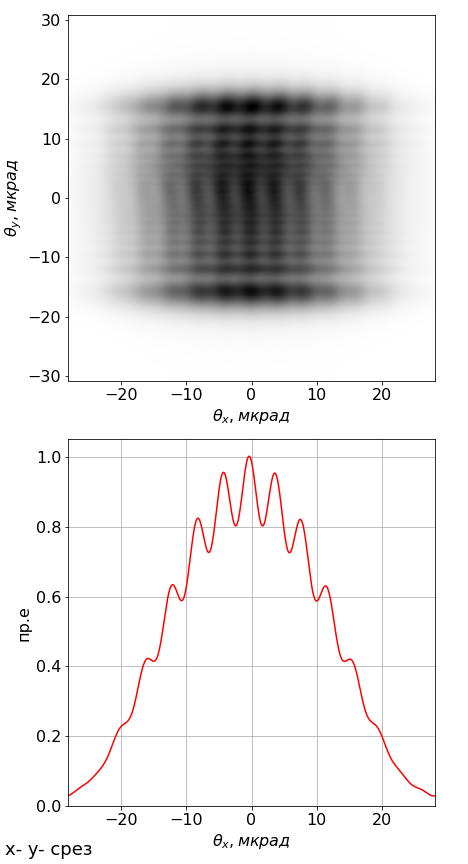
\includegraphics[width=1\linewidth]{x_slits_width_3e-05_separation_0.00015_.png}
		\caption{}
		\label{fig:2-beam_size_s}
	\end{minipage}\hfill
	\begin{minipage}{0.33\textwidth}
		\centering
		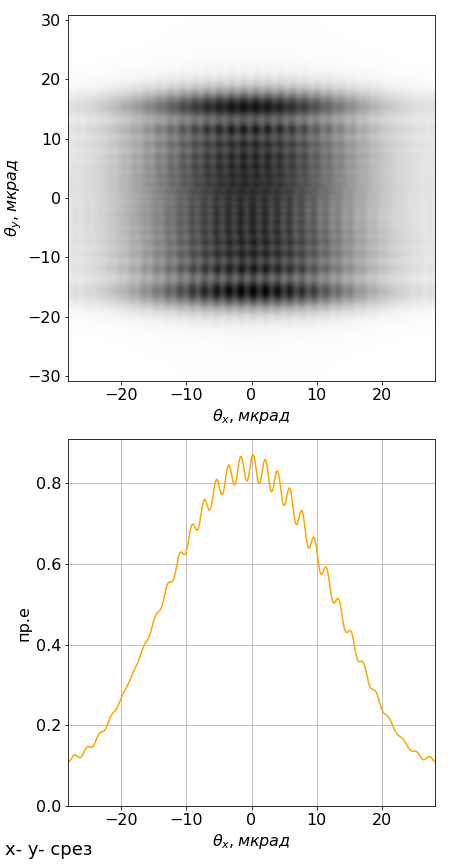
\includegraphics[width=1\linewidth]{x_slits_width_3e-05_separation_0.0003_.png}
		\caption{}
		\label{fig:2-beam_size_s}
	\end{minipage}\hfill
\end{figure}

\begin{figure}[H]
	\centering
	\begin{minipage}{0.33\textwidth}
		\centering
		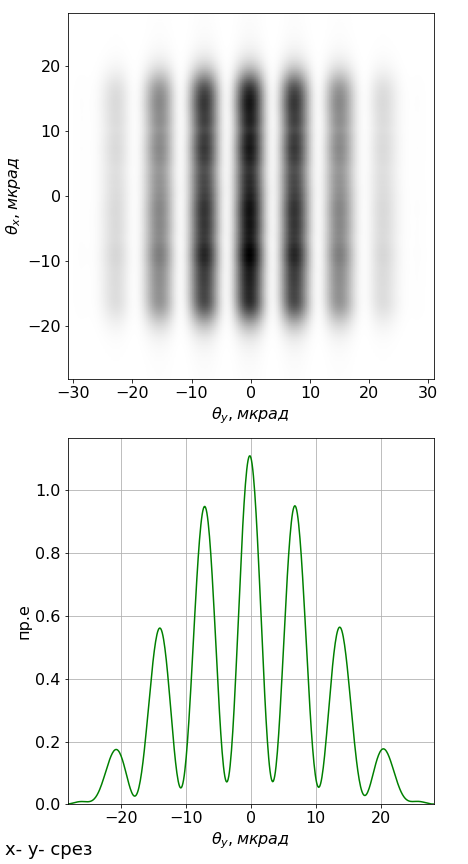
\includegraphics[width=1\linewidth]{y_slits_width_3e-05_separation_7.5e-05_.png}
		\caption{}
		\label{fig:2-beam_size_k}
	\end{minipage}
	\begin{minipage}{0.33\textwidth}
		\centering
		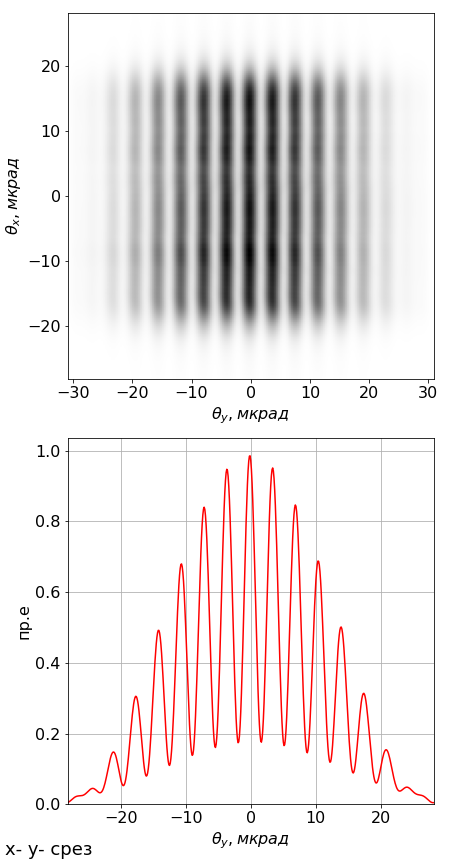
\includegraphics[width=1\linewidth]{y_slits_width_3e-05_separation_0.00015_.png}
		\caption{}
		\label{fig:2-beam_size_s}
	\end{minipage}\hfill
	\begin{minipage}{0.33\textwidth}
		\centering
		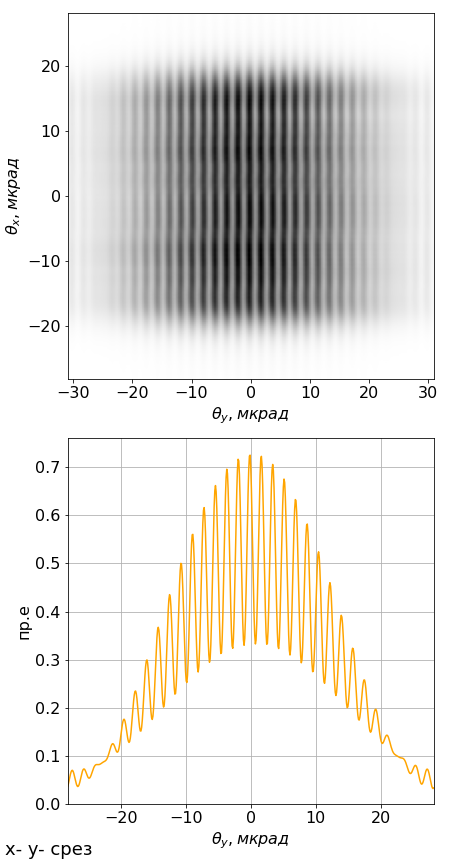
\includegraphics[width=1\linewidth]{y_slits_width_3e-05_separation_0.0003_.png}
		\caption{}
		\label{fig:2-beam_size_s}
\end{minipage}\hfill
\end{figure}


\subsection{Отражение от неидеального зеркала}






